\documentclass[11pt]{article}
\usepackage[textwidth=18.0cm, textheight=23.0cm, top=2.0cm]{geometry}
\usepackage{pst-all}
\usepackage{amssymb}
\usepackage{tikz}
\usepackage{underscore}\begin{document}
\pagestyle{empty}


ClassName: \underline{\textbf{Class_07.2bp-30}}
\par
BinSize: \underline{\textbf{100 × 100}}
\par
ReduceSize: \underline{\textbf{100 × 100}}
\par
TypeNum: \underline{\textbf{77}}
\par
Num: \underline{\textbf{80}}
\par
OutS: \underline{\textbf{210000}}
\par
InS: \underline{\textbf{179454}}
\par
Rate: \underline{\textbf{0.855}}
\par
UB: \underline{\textbf{21}}
\par
LB0: \underline{\textbf{20}}
\par
LB: \underline{\textbf{21}}
\par
LBWithCut: \underline{\textbf{21}}
\par
NodeCut: \underline{\textbf{0}}
\par
ExtendedNodeCnt: \underline{\textbf{1}}
\par
GenNodeCnt: \underline{\textbf{1}}
\par
PrimalNode: \underline{\textbf{0}}
\par
ColumnCount: \underline{\textbf{228}}
\par
TotalCutCount: \underline{\textbf{0}}
\par
RootCutCount: \underline{\textbf{0}}
\par
LPSolverCnt: \underline{\textbf{208}}
\par
PricingSolverCnt: \underline{\textbf{208}}
\par
BranchAndBoundNum: \underline{\textbf{1}}
\par
isOpt: \underline{\textbf{true}}
\par
TimeOnInitSolution: \underline{\textbf{120.020 s}}
\par
TimeOnPrimal: \underline{\textbf{0.000 s}}
\par
TimeOnPricing: \underline{\textbf{29.000 s}}
\par
TimeOnRmp: \underline{\textbf{0.126 s}}
\par
TotalTime: \underline{\textbf{149.347 s}}
\par
\newpage


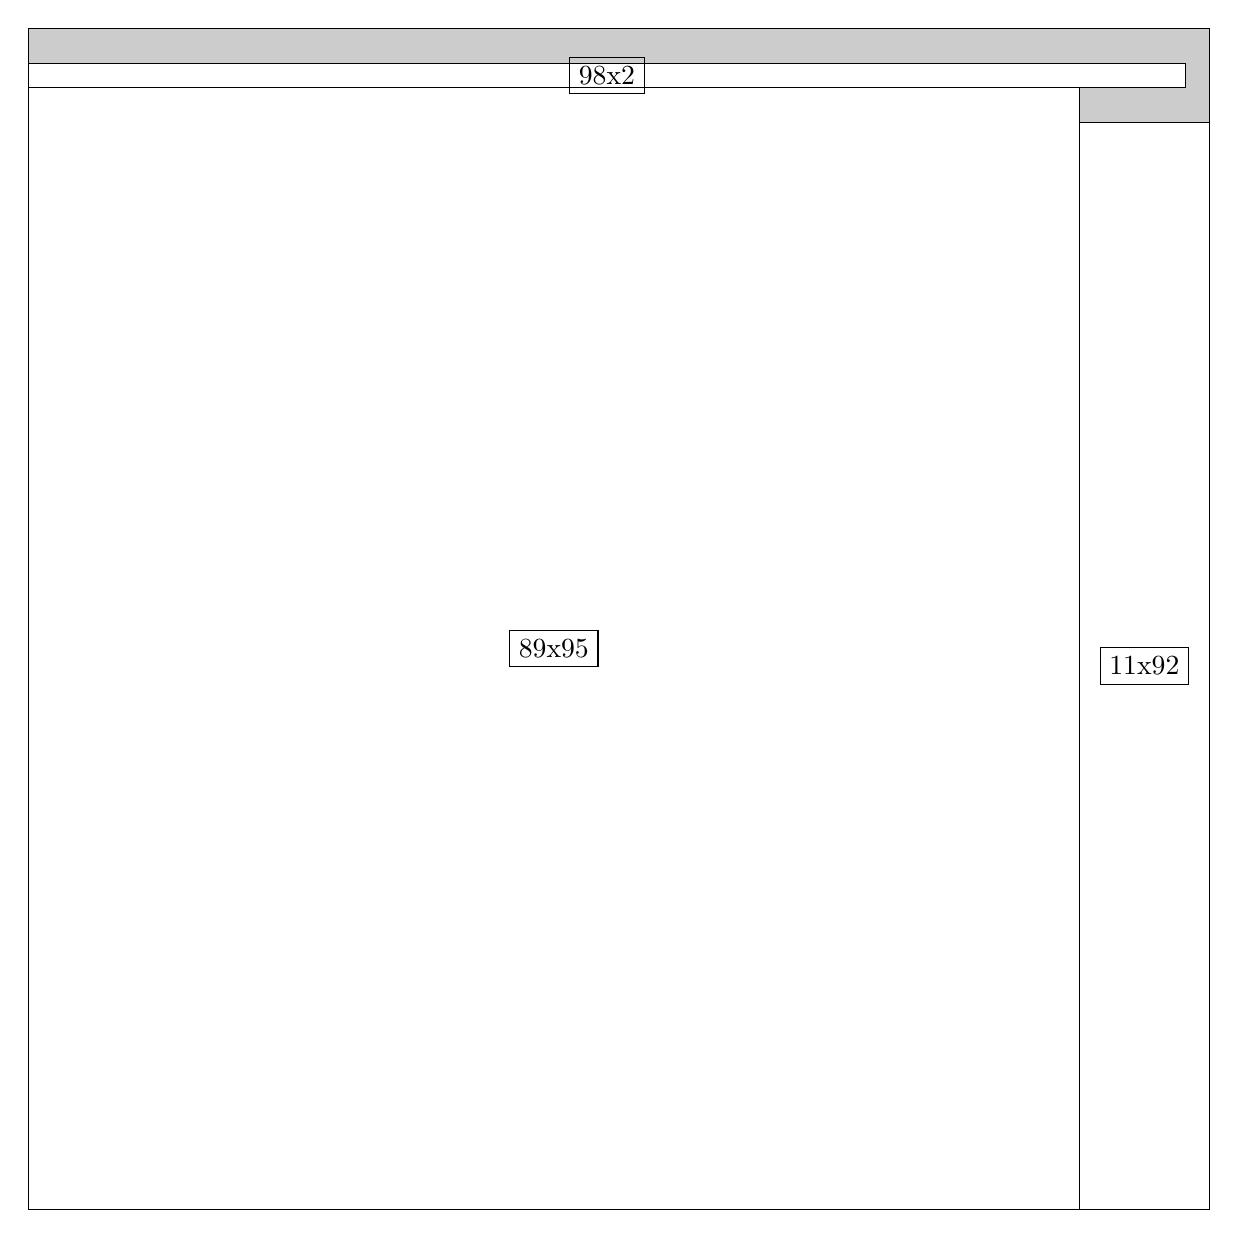
\begin{tikzpicture}[shorten >=1pt,scale=1.0,every node/.style={scale=1.0},->]
\tikzstyle{vertex}=[circle,fill=black!25,minimum size=14pt,inner sep=0pt]
\filldraw[fill=gray!40!white, draw=black] (0,0) rectangle (15.0,15.0);
\foreach \name/\x/\y/\w/\h in {89x95/0.0/0.0/13.35/14.25,98x2/0.0/14.25/14.7/0.3,11x92/13.35/0.0/1.65/13.799999999999999}
\filldraw[fill=white!40!white, draw=black] (\x,\y) rectangle node[draw] (\name) {\name} ++(\w,\h);
\end{tikzpicture}


w =89 , h =95 , x =0 , y =0 , v =8455
\par
w =98 , h =2 , x =0 , y =95 , v =196
\par
w =11 , h =92 , x =89 , y =0 , v =1012
\par
\newpage


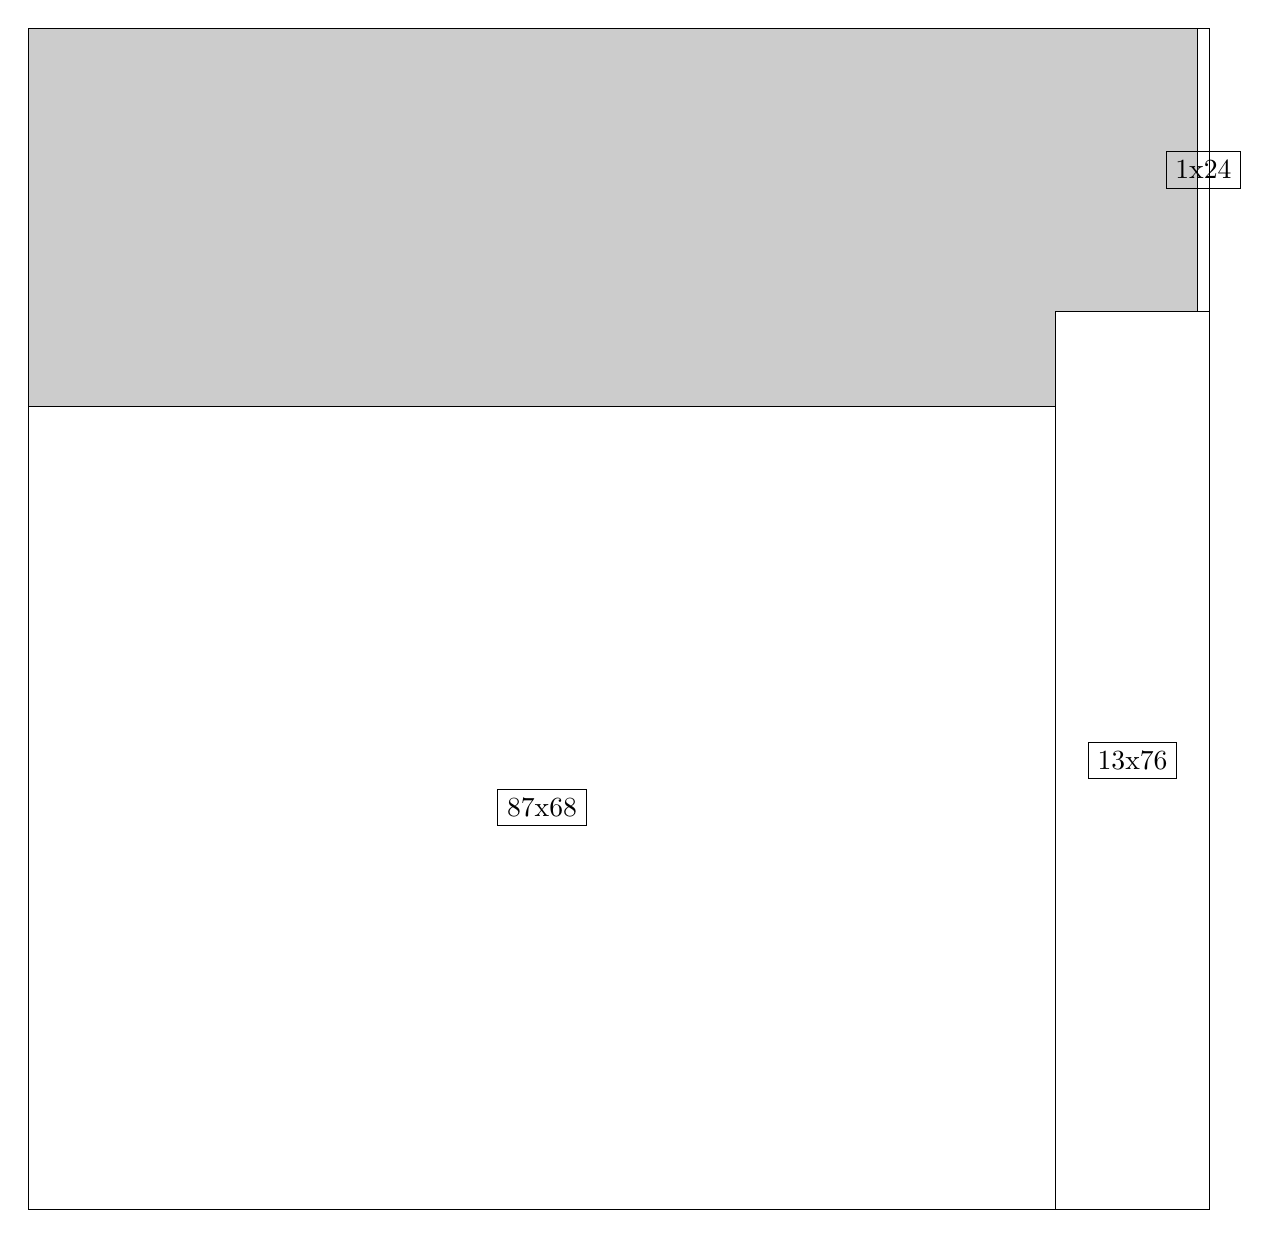
\begin{tikzpicture}[shorten >=1pt,scale=1.0,every node/.style={scale=1.0},->]
\tikzstyle{vertex}=[circle,fill=black!25,minimum size=14pt,inner sep=0pt]
\filldraw[fill=gray!40!white, draw=black] (0,0) rectangle (15.0,15.0);
\foreach \name/\x/\y/\w/\h in {87x68/0.0/0.0/13.049999999999999/10.2,13x76/13.049999999999999/0.0/1.95/11.4,1x24/14.85/11.4/0.15/3.5999999999999996}
\filldraw[fill=white!40!white, draw=black] (\x,\y) rectangle node[draw] (\name) {\name} ++(\w,\h);
\end{tikzpicture}


w =87 , h =68 , x =0 , y =0 , v =5916
\par
w =13 , h =76 , x =87 , y =0 , v =988
\par
w =1 , h =24 , x =99 , y =76 , v =24
\par
\newpage


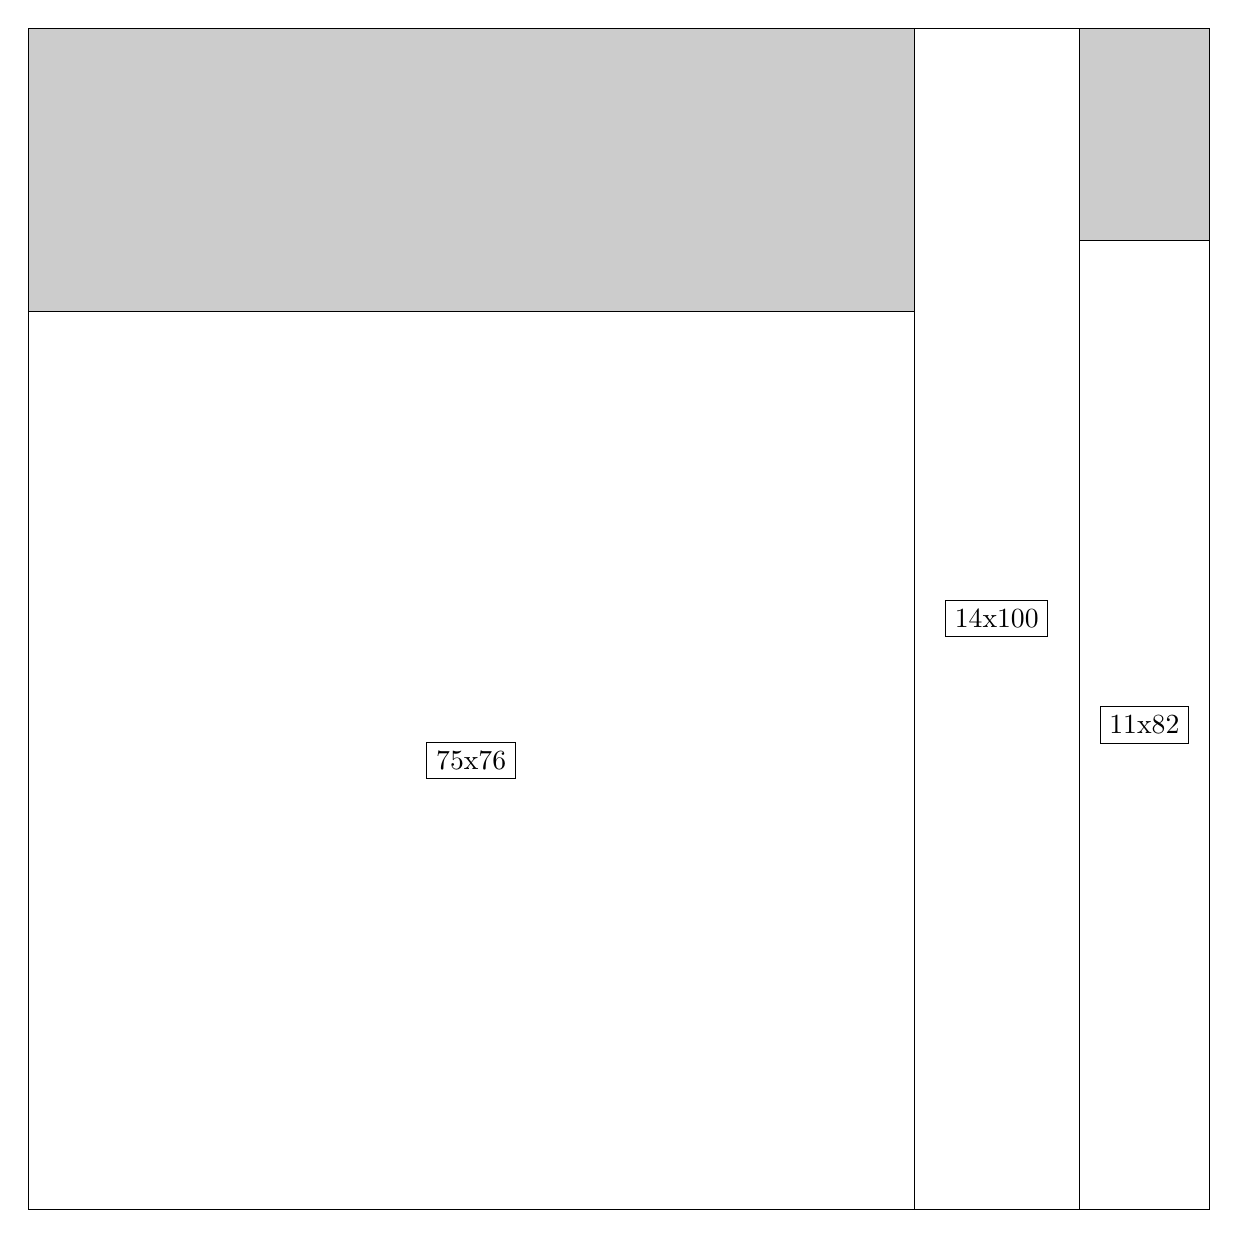
\begin{tikzpicture}[shorten >=1pt,scale=1.0,every node/.style={scale=1.0},->]
\tikzstyle{vertex}=[circle,fill=black!25,minimum size=14pt,inner sep=0pt]
\filldraw[fill=gray!40!white, draw=black] (0,0) rectangle (15.0,15.0);
\foreach \name/\x/\y/\w/\h in {75x76/0.0/0.0/11.25/11.4,11x82/13.35/0.0/1.65/12.299999999999999,14x100/11.25/0.0/2.1/15.0}
\filldraw[fill=white!40!white, draw=black] (\x,\y) rectangle node[draw] (\name) {\name} ++(\w,\h);
\end{tikzpicture}


w =75 , h =76 , x =0 , y =0 , v =5700
\par
w =11 , h =82 , x =89 , y =0 , v =902
\par
w =14 , h =100 , x =75 , y =0 , v =1400
\par
\newpage


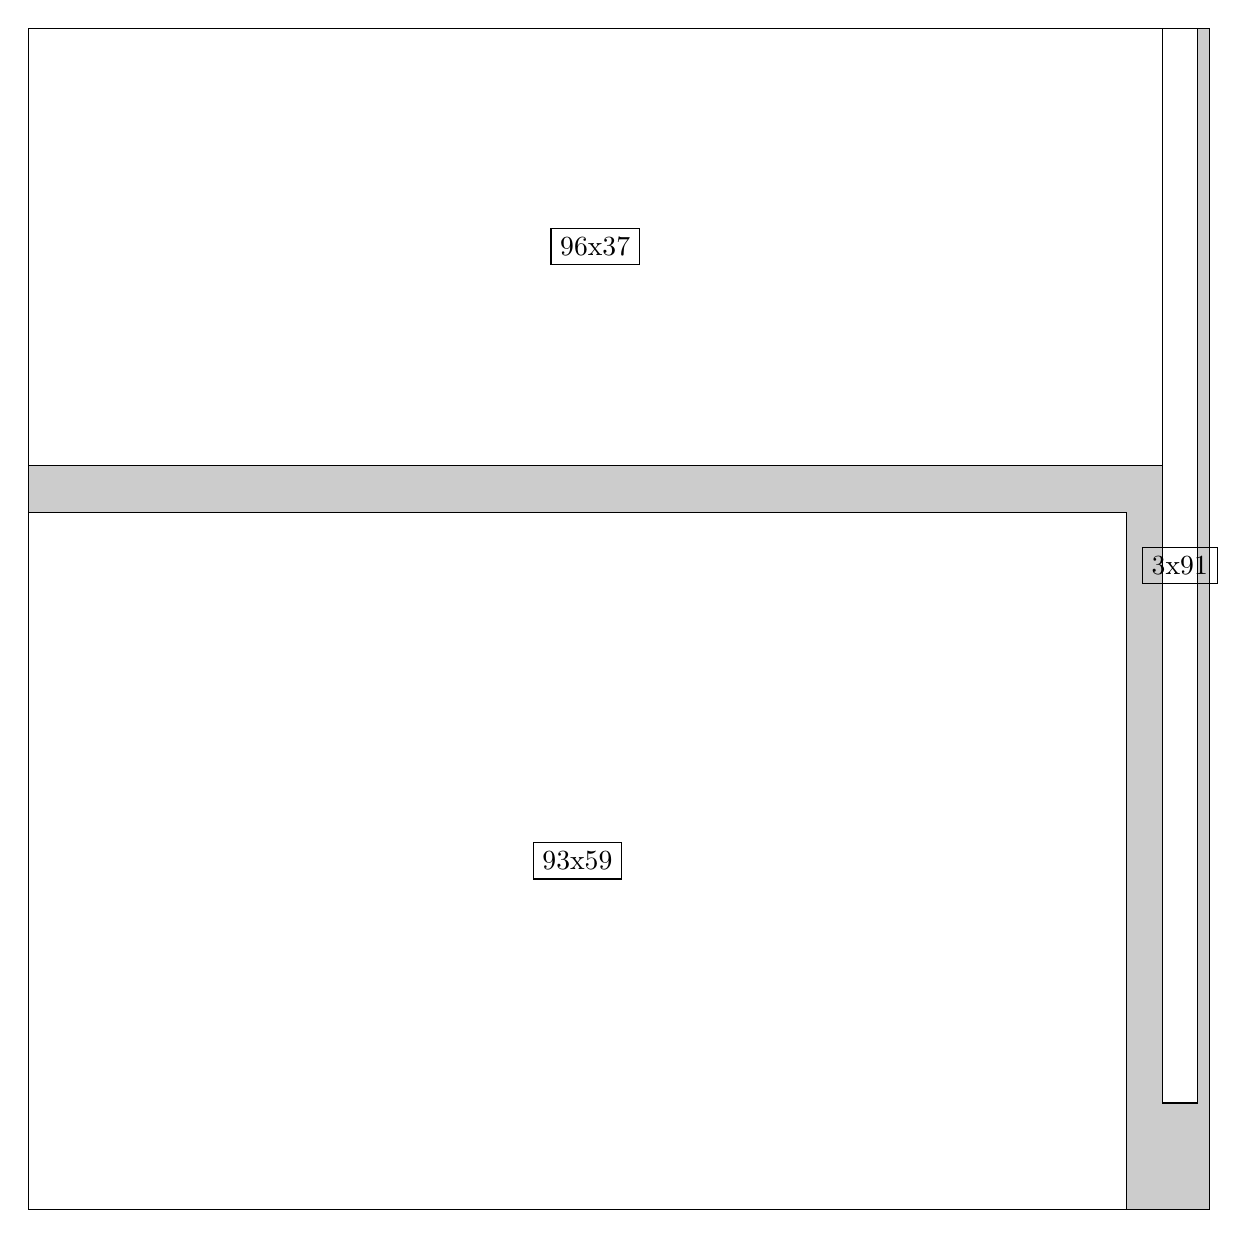
\begin{tikzpicture}[shorten >=1pt,scale=1.0,every node/.style={scale=1.0},->]
\tikzstyle{vertex}=[circle,fill=black!25,minimum size=14pt,inner sep=0pt]
\filldraw[fill=gray!40!white, draw=black] (0,0) rectangle (15.0,15.0);
\foreach \name/\x/\y/\w/\h in {93x59/0.0/0.0/13.95/8.85,96x37/0.0/9.45/14.399999999999999/5.55,3x91/14.399999999999999/1.3499999999999999/0.44999999999999996/13.65}
\filldraw[fill=white!40!white, draw=black] (\x,\y) rectangle node[draw] (\name) {\name} ++(\w,\h);
\end{tikzpicture}


w =93 , h =59 , x =0 , y =0 , v =5487
\par
w =96 , h =37 , x =0 , y =63 , v =3552
\par
w =3 , h =91 , x =96 , y =9 , v =273
\par
\newpage


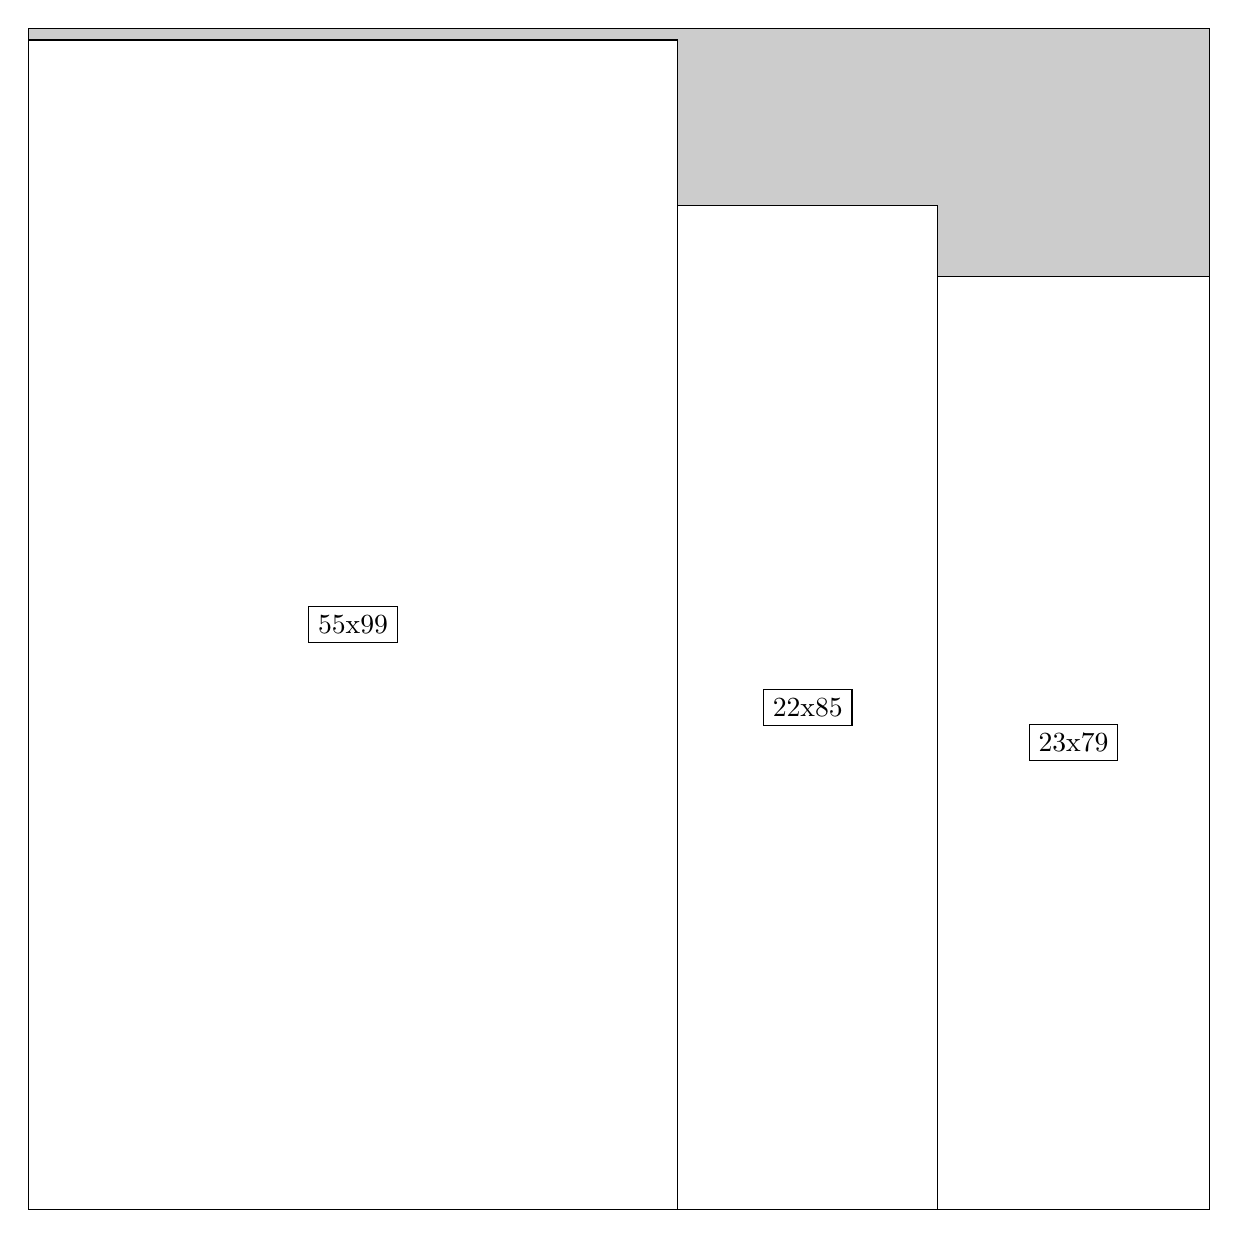
\begin{tikzpicture}[shorten >=1pt,scale=1.0,every node/.style={scale=1.0},->]
\tikzstyle{vertex}=[circle,fill=black!25,minimum size=14pt,inner sep=0pt]
\filldraw[fill=gray!40!white, draw=black] (0,0) rectangle (15.0,15.0);
\foreach \name/\x/\y/\w/\h in {55x99/0.0/0.0/8.25/14.85,22x85/8.25/0.0/3.3/12.75,23x79/11.549999999999999/0.0/3.4499999999999997/11.85}
\filldraw[fill=white!40!white, draw=black] (\x,\y) rectangle node[draw] (\name) {\name} ++(\w,\h);
\end{tikzpicture}


w =55 , h =99 , x =0 , y =0 , v =5445
\par
w =22 , h =85 , x =55 , y =0 , v =1870
\par
w =23 , h =79 , x =77 , y =0 , v =1817
\par
\newpage


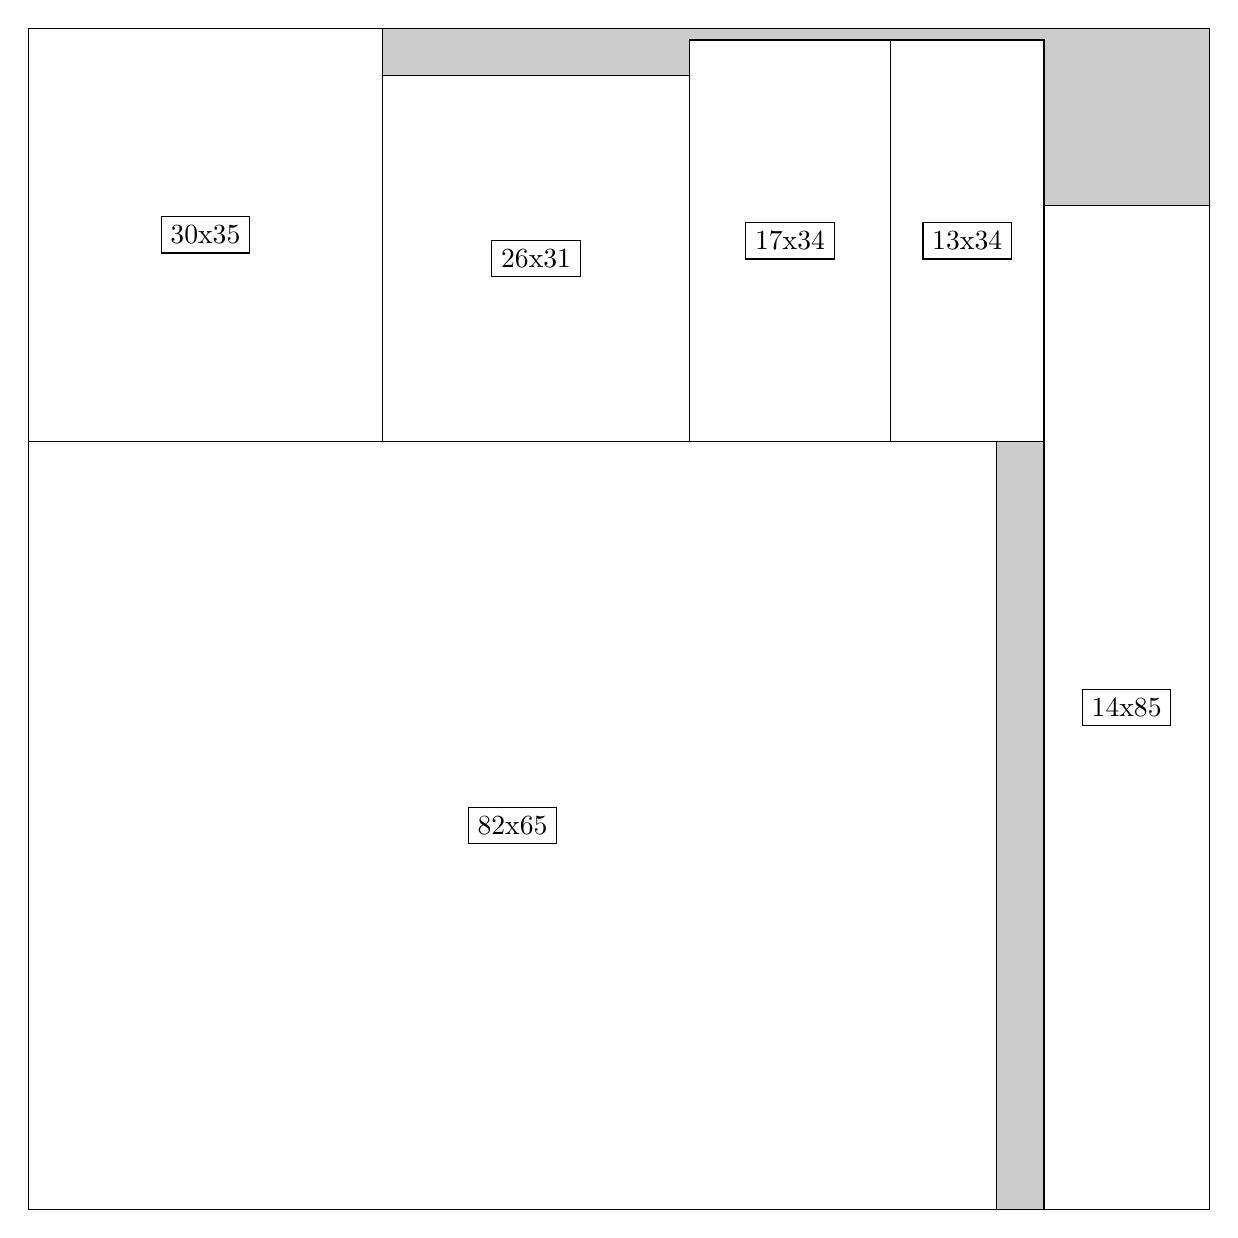
\begin{tikzpicture}[shorten >=1pt,scale=1.0,every node/.style={scale=1.0},->]
\tikzstyle{vertex}=[circle,fill=black!25,minimum size=14pt,inner sep=0pt]
\filldraw[fill=gray!40!white, draw=black] (0,0) rectangle (15.0,15.0);
\foreach \name/\x/\y/\w/\h in {82x65/0.0/0.0/12.299999999999999/9.75,14x85/12.9/0.0/2.1/12.75,30x35/0.0/9.75/4.5/5.25,26x31/4.5/9.75/3.9/4.6499999999999995,17x34/8.4/9.75/2.55/5.1,13x34/10.95/9.75/1.95/5.1}
\filldraw[fill=white!40!white, draw=black] (\x,\y) rectangle node[draw] (\name) {\name} ++(\w,\h);
\end{tikzpicture}


w =82 , h =65 , x =0 , y =0 , v =5330
\par
w =14 , h =85 , x =86 , y =0 , v =1190
\par
w =30 , h =35 , x =0 , y =65 , v =1050
\par
w =26 , h =31 , x =30 , y =65 , v =806
\par
w =17 , h =34 , x =56 , y =65 , v =578
\par
w =13 , h =34 , x =73 , y =65 , v =442
\par
\newpage


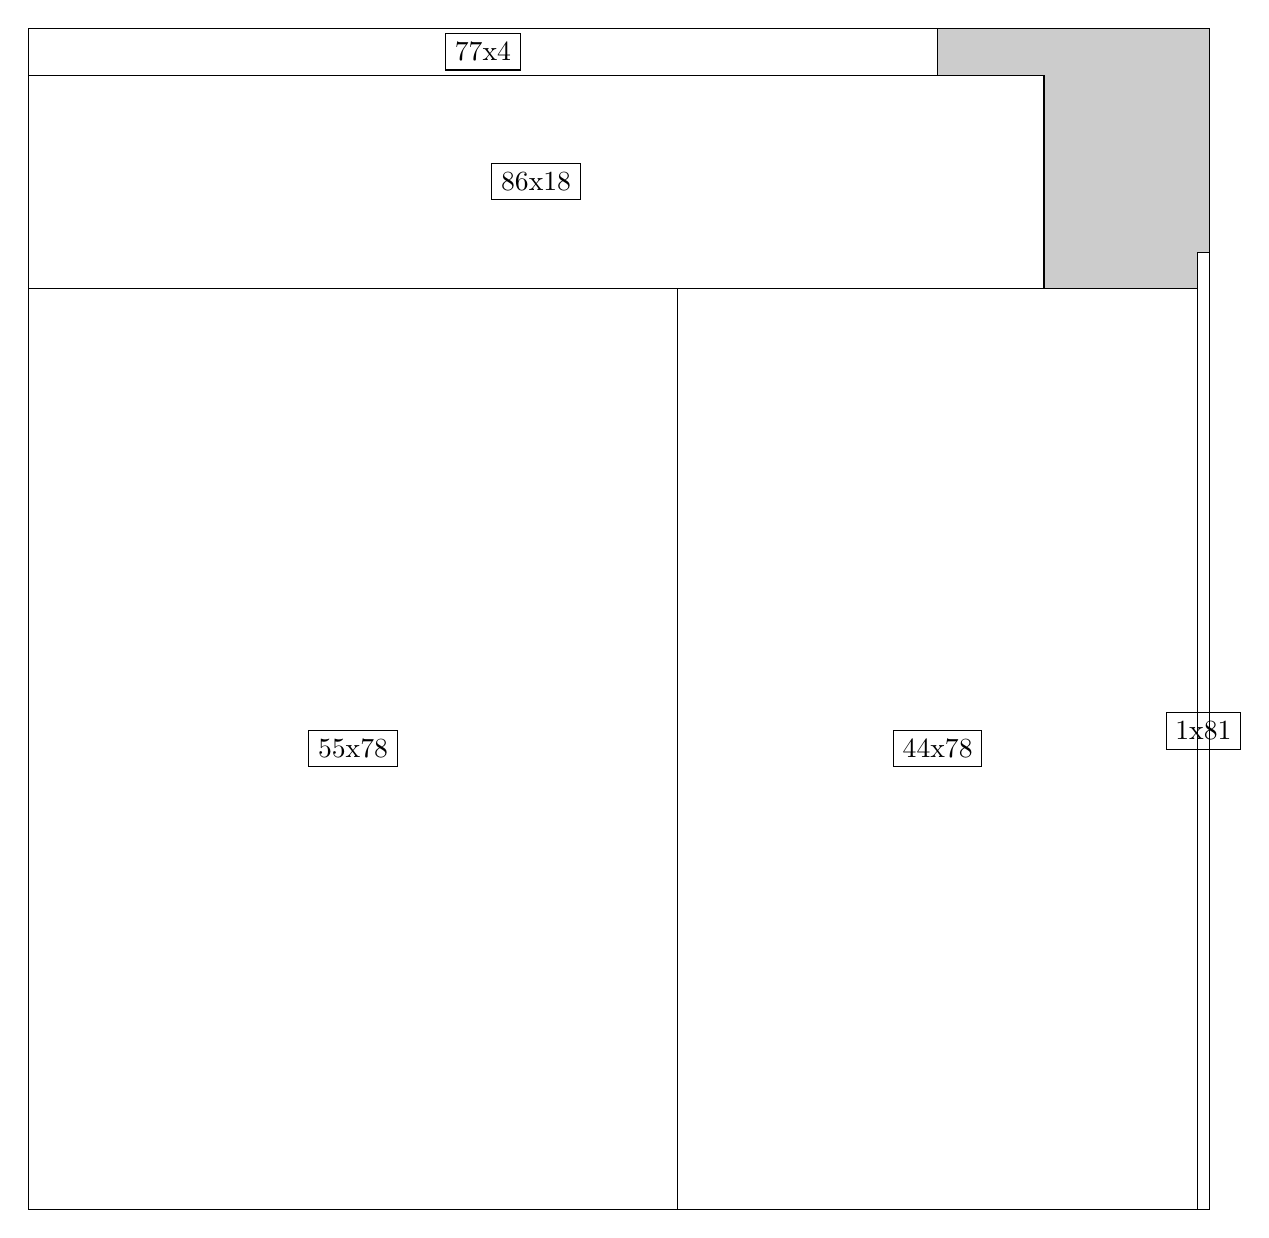
\begin{tikzpicture}[shorten >=1pt,scale=1.0,every node/.style={scale=1.0},->]
\tikzstyle{vertex}=[circle,fill=black!25,minimum size=14pt,inner sep=0pt]
\filldraw[fill=gray!40!white, draw=black] (0,0) rectangle (15.0,15.0);
\foreach \name/\x/\y/\w/\h in {55x78/0.0/0.0/8.25/11.7,44x78/8.25/0.0/6.6/11.7,86x18/0.0/11.7/12.9/2.6999999999999997,77x4/0.0/14.399999999999999/11.549999999999999/0.6,1x81/14.85/0.0/0.15/12.15}
\filldraw[fill=white!40!white, draw=black] (\x,\y) rectangle node[draw] (\name) {\name} ++(\w,\h);
\end{tikzpicture}


w =55 , h =78 , x =0 , y =0 , v =4290
\par
w =44 , h =78 , x =55 , y =0 , v =3432
\par
w =86 , h =18 , x =0 , y =78 , v =1548
\par
w =77 , h =4 , x =0 , y =96 , v =308
\par
w =1 , h =81 , x =99 , y =0 , v =81
\par
\newpage


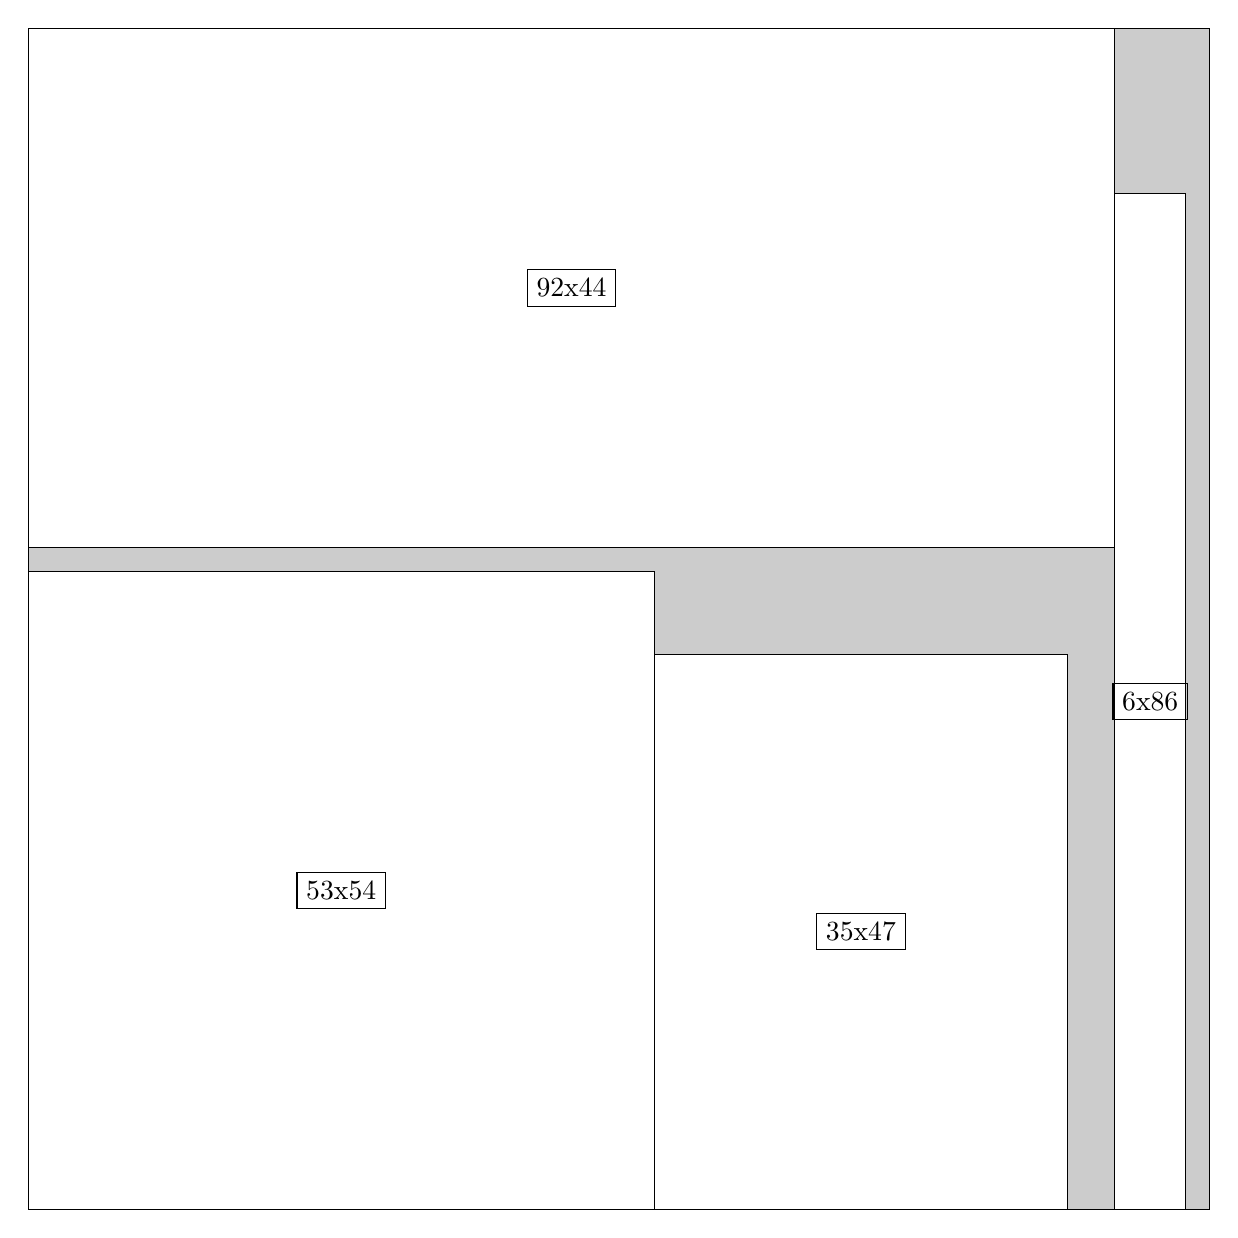
\begin{tikzpicture}[shorten >=1pt,scale=1.0,every node/.style={scale=1.0},->]
\tikzstyle{vertex}=[circle,fill=black!25,minimum size=14pt,inner sep=0pt]
\filldraw[fill=gray!40!white, draw=black] (0,0) rectangle (15.0,15.0);
\foreach \name/\x/\y/\w/\h in {92x44/0.0/8.4/13.799999999999999/6.6,53x54/0.0/0.0/7.949999999999999/8.1,35x47/7.949999999999999/0.0/5.25/7.05,6x86/13.799999999999999/0.0/0.8999999999999999/12.9}
\filldraw[fill=white!40!white, draw=black] (\x,\y) rectangle node[draw] (\name) {\name} ++(\w,\h);
\end{tikzpicture}


w =92 , h =44 , x =0 , y =56 , v =4048
\par
w =53 , h =54 , x =0 , y =0 , v =2862
\par
w =35 , h =47 , x =53 , y =0 , v =1645
\par
w =6 , h =86 , x =92 , y =0 , v =516
\par
\newpage


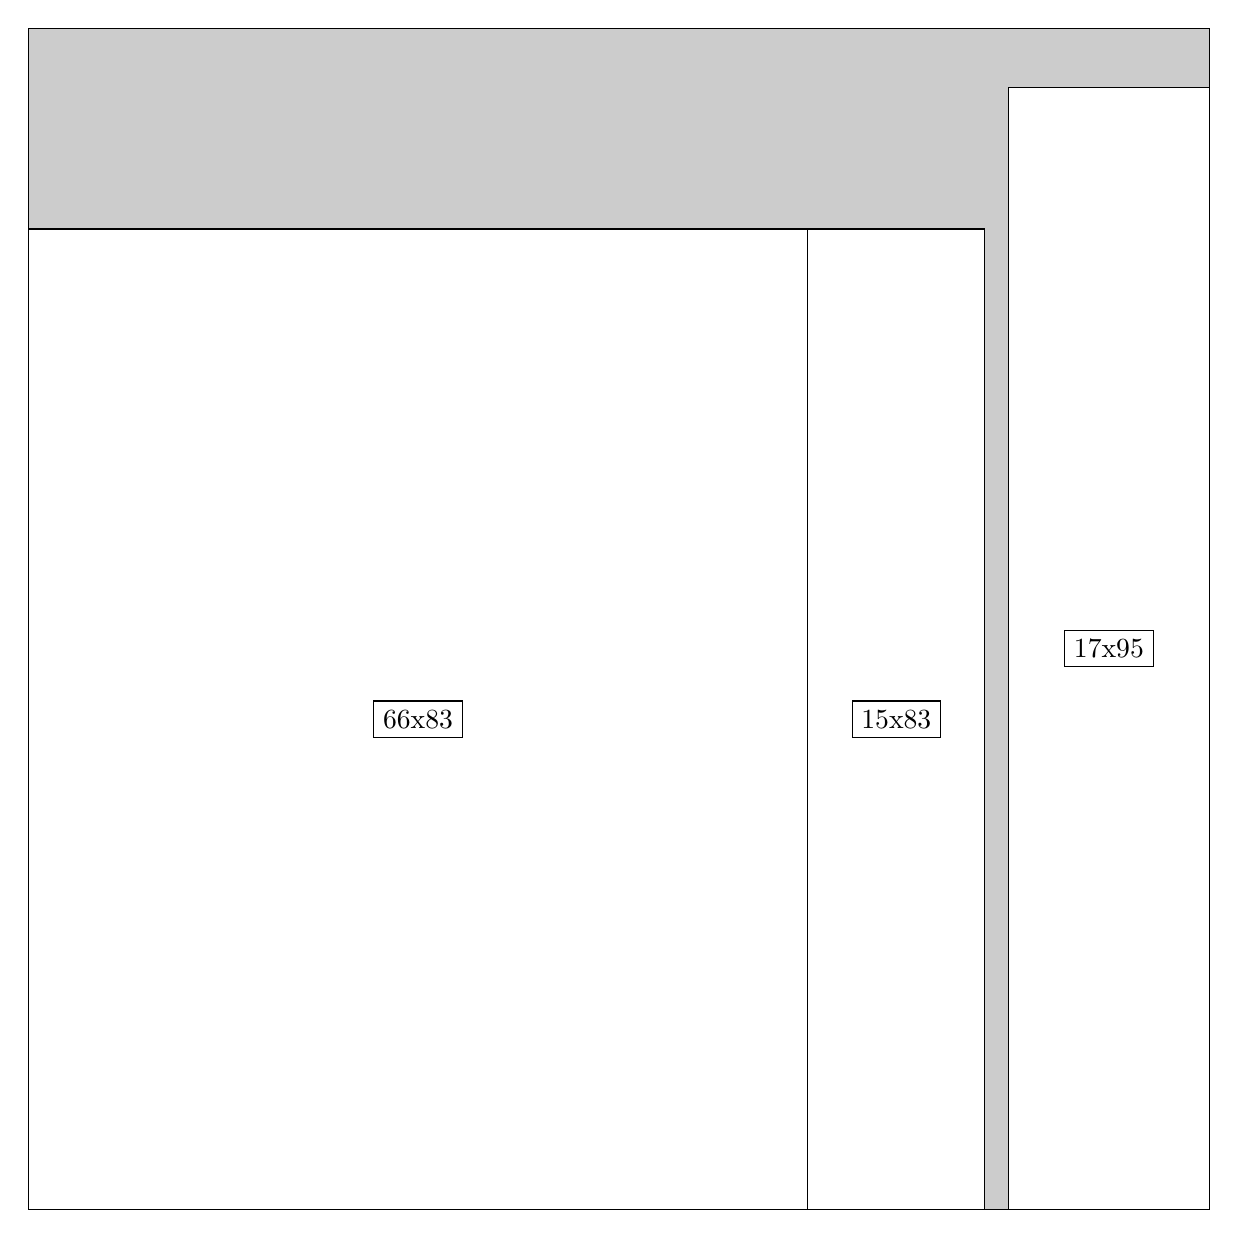
\begin{tikzpicture}[shorten >=1pt,scale=1.0,every node/.style={scale=1.0},->]
\tikzstyle{vertex}=[circle,fill=black!25,minimum size=14pt,inner sep=0pt]
\filldraw[fill=gray!40!white, draw=black] (0,0) rectangle (15.0,15.0);
\foreach \name/\x/\y/\w/\h in {66x83/0.0/0.0/9.9/12.45,17x95/12.45/0.0/2.55/14.25,15x83/9.9/0.0/2.25/12.45}
\filldraw[fill=white!40!white, draw=black] (\x,\y) rectangle node[draw] (\name) {\name} ++(\w,\h);
\end{tikzpicture}


w =66 , h =83 , x =0 , y =0 , v =5478
\par
w =17 , h =95 , x =83 , y =0 , v =1615
\par
w =15 , h =83 , x =66 , y =0 , v =1245
\par
\newpage


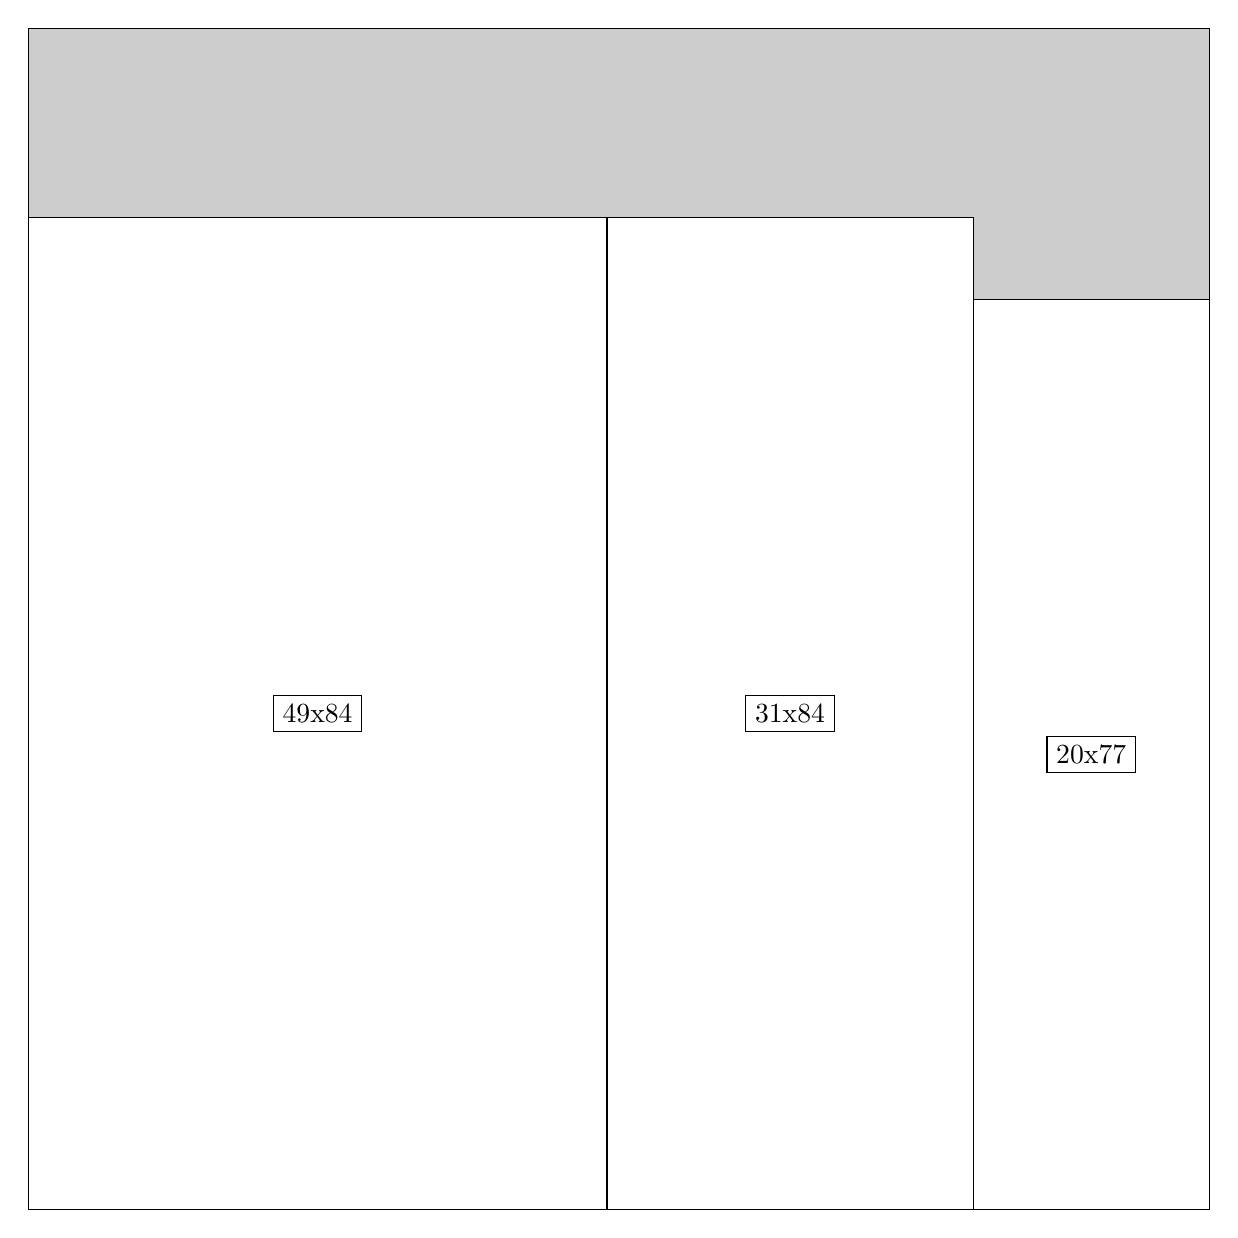
\begin{tikzpicture}[shorten >=1pt,scale=1.0,every node/.style={scale=1.0},->]
\tikzstyle{vertex}=[circle,fill=black!25,minimum size=14pt,inner sep=0pt]
\filldraw[fill=gray!40!white, draw=black] (0,0) rectangle (15.0,15.0);
\foreach \name/\x/\y/\w/\h in {49x84/0.0/0.0/7.35/12.6,31x84/7.35/0.0/4.6499999999999995/12.6,20x77/12.0/0.0/3.0/11.549999999999999}
\filldraw[fill=white!40!white, draw=black] (\x,\y) rectangle node[draw] (\name) {\name} ++(\w,\h);
\end{tikzpicture}


w =49 , h =84 , x =0 , y =0 , v =4116
\par
w =31 , h =84 , x =49 , y =0 , v =2604
\par
w =20 , h =77 , x =80 , y =0 , v =1540
\par
\newpage


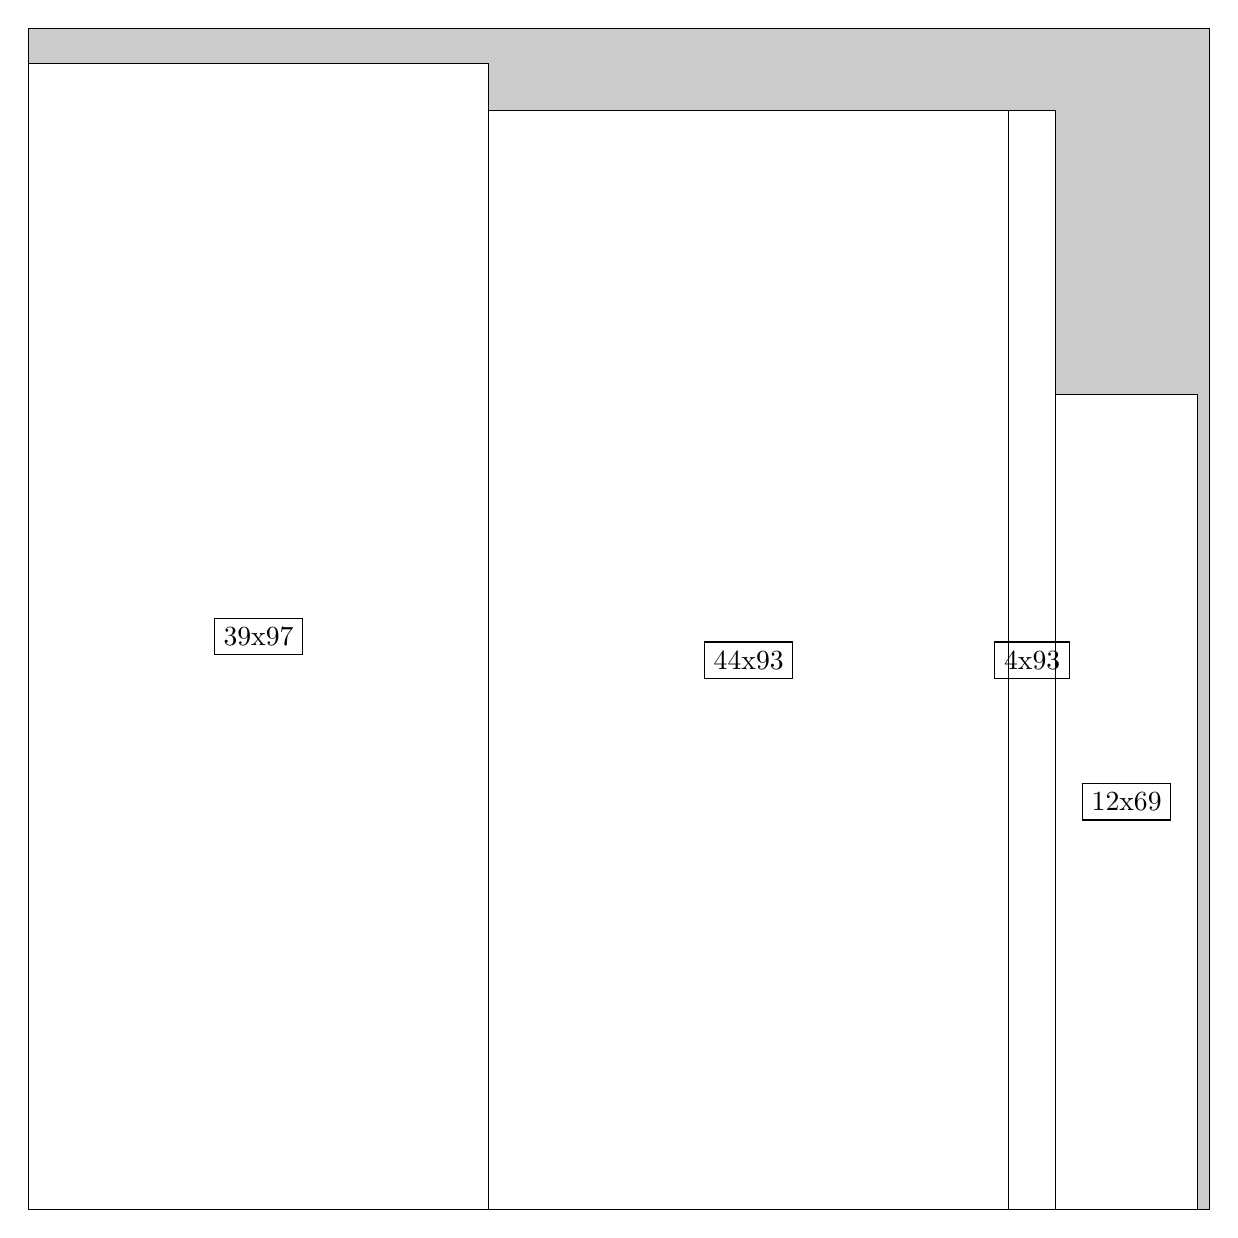
\begin{tikzpicture}[shorten >=1pt,scale=1.0,every node/.style={scale=1.0},->]
\tikzstyle{vertex}=[circle,fill=black!25,minimum size=14pt,inner sep=0pt]
\filldraw[fill=gray!40!white, draw=black] (0,0) rectangle (15.0,15.0);
\foreach \name/\x/\y/\w/\h in {44x93/5.85/0.0/6.6/13.95,39x97/0.0/0.0/5.85/14.549999999999999,12x69/13.049999999999999/0.0/1.7999999999999998/10.35,4x93/12.45/0.0/0.6/13.95}
\filldraw[fill=white!40!white, draw=black] (\x,\y) rectangle node[draw] (\name) {\name} ++(\w,\h);
\end{tikzpicture}


w =44 , h =93 , x =39 , y =0 , v =4092
\par
w =39 , h =97 , x =0 , y =0 , v =3783
\par
w =12 , h =69 , x =87 , y =0 , v =828
\par
w =4 , h =93 , x =83 , y =0 , v =372
\par
\newpage


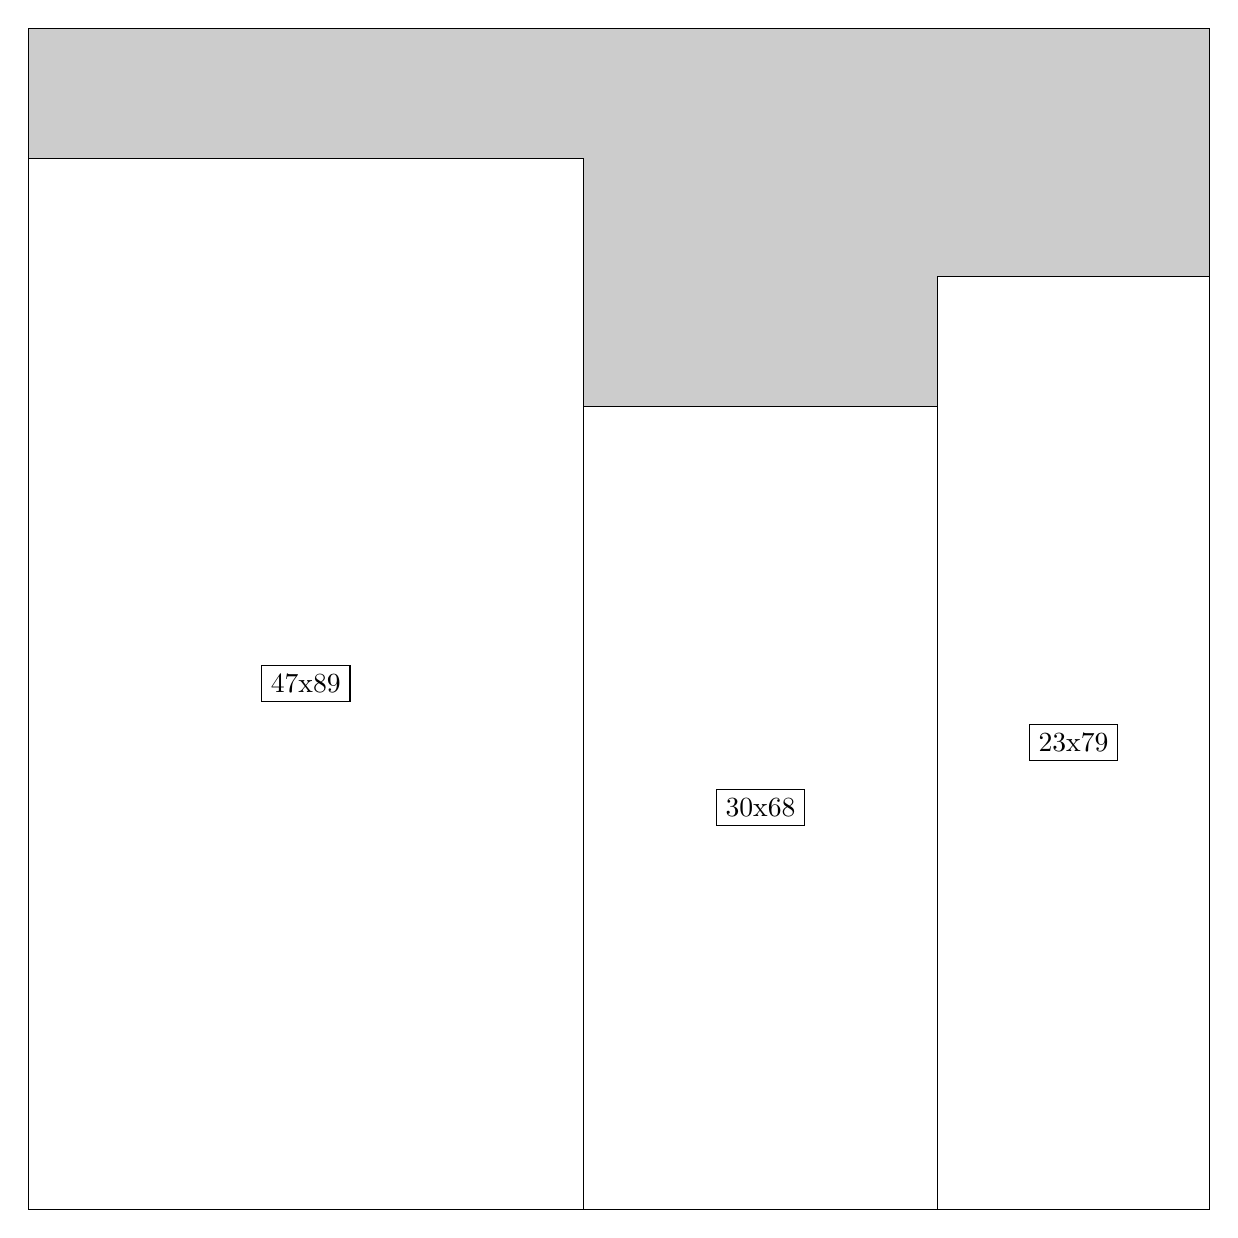
\begin{tikzpicture}[shorten >=1pt,scale=1.0,every node/.style={scale=1.0},->]
\tikzstyle{vertex}=[circle,fill=black!25,minimum size=14pt,inner sep=0pt]
\filldraw[fill=gray!40!white, draw=black] (0,0) rectangle (15.0,15.0);
\foreach \name/\x/\y/\w/\h in {47x89/0.0/0.0/7.05/13.35,30x68/7.05/0.0/4.5/10.2,23x79/11.549999999999999/0.0/3.4499999999999997/11.85}
\filldraw[fill=white!40!white, draw=black] (\x,\y) rectangle node[draw] (\name) {\name} ++(\w,\h);
\end{tikzpicture}


w =47 , h =89 , x =0 , y =0 , v =4183
\par
w =30 , h =68 , x =47 , y =0 , v =2040
\par
w =23 , h =79 , x =77 , y =0 , v =1817
\par
\newpage


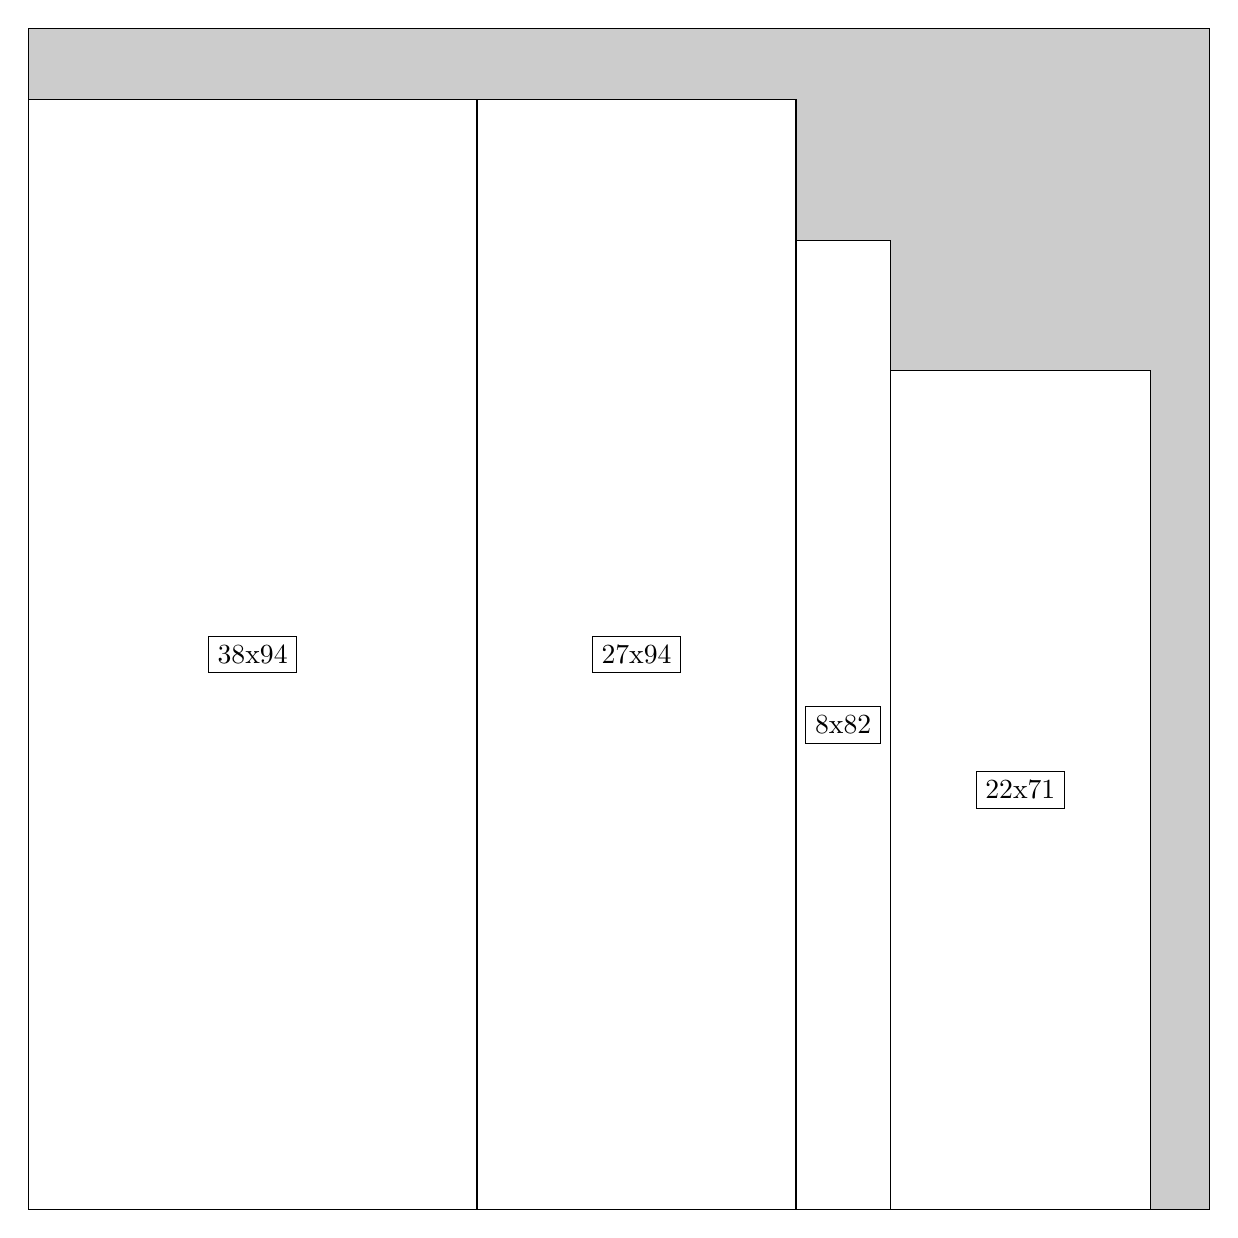
\begin{tikzpicture}[shorten >=1pt,scale=1.0,every node/.style={scale=1.0},->]
\tikzstyle{vertex}=[circle,fill=black!25,minimum size=14pt,inner sep=0pt]
\filldraw[fill=gray!40!white, draw=black] (0,0) rectangle (15.0,15.0);
\foreach \name/\x/\y/\w/\h in {38x94/0.0/0.0/5.7/14.1,27x94/5.7/0.0/4.05/14.1,22x71/10.95/0.0/3.3/10.65,8x82/9.75/0.0/1.2/12.299999999999999}
\filldraw[fill=white!40!white, draw=black] (\x,\y) rectangle node[draw] (\name) {\name} ++(\w,\h);
\end{tikzpicture}


w =38 , h =94 , x =0 , y =0 , v =3572
\par
w =27 , h =94 , x =38 , y =0 , v =2538
\par
w =22 , h =71 , x =73 , y =0 , v =1562
\par
w =8 , h =82 , x =65 , y =0 , v =656
\par
\newpage


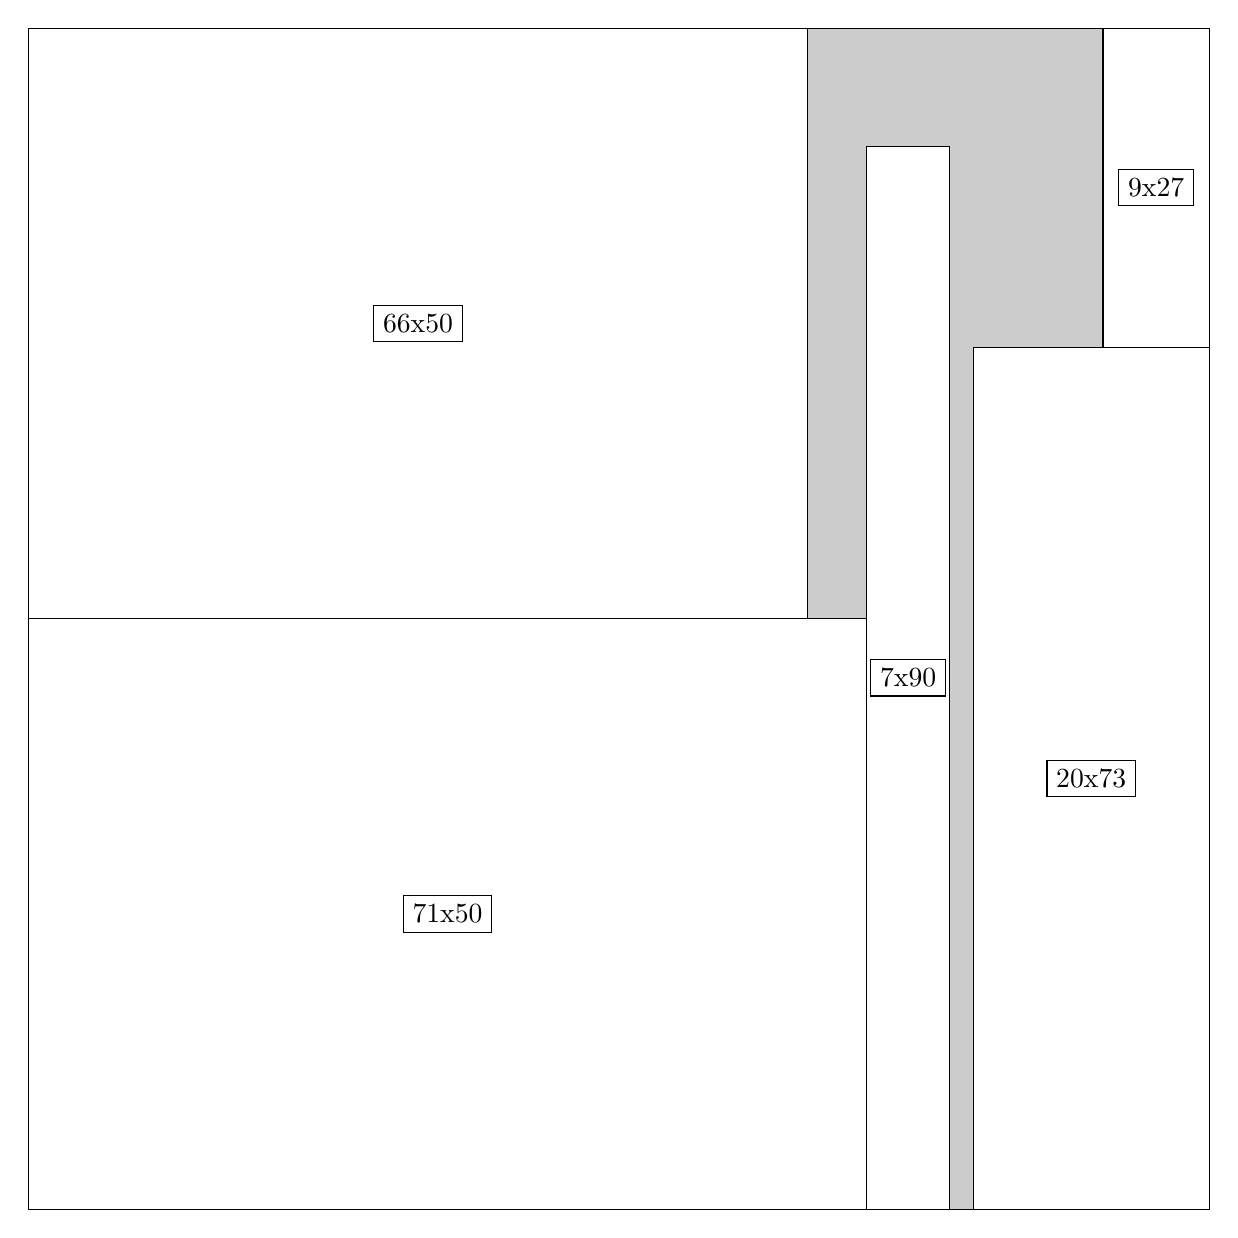
\begin{tikzpicture}[shorten >=1pt,scale=1.0,every node/.style={scale=1.0},->]
\tikzstyle{vertex}=[circle,fill=black!25,minimum size=14pt,inner sep=0pt]
\filldraw[fill=gray!40!white, draw=black] (0,0) rectangle (15.0,15.0);
\foreach \name/\x/\y/\w/\h in {71x50/0.0/0.0/10.65/7.5,66x50/0.0/7.5/9.9/7.5,20x73/12.0/0.0/3.0/10.95,7x90/10.65/0.0/1.05/13.5,9x27/13.65/10.95/1.3499999999999999/4.05}
\filldraw[fill=white!40!white, draw=black] (\x,\y) rectangle node[draw] (\name) {\name} ++(\w,\h);
\end{tikzpicture}


w =71 , h =50 , x =0 , y =0 , v =3550
\par
w =66 , h =50 , x =0 , y =50 , v =3300
\par
w =20 , h =73 , x =80 , y =0 , v =1460
\par
w =7 , h =90 , x =71 , y =0 , v =630
\par
w =9 , h =27 , x =91 , y =73 , v =243
\par
\newpage


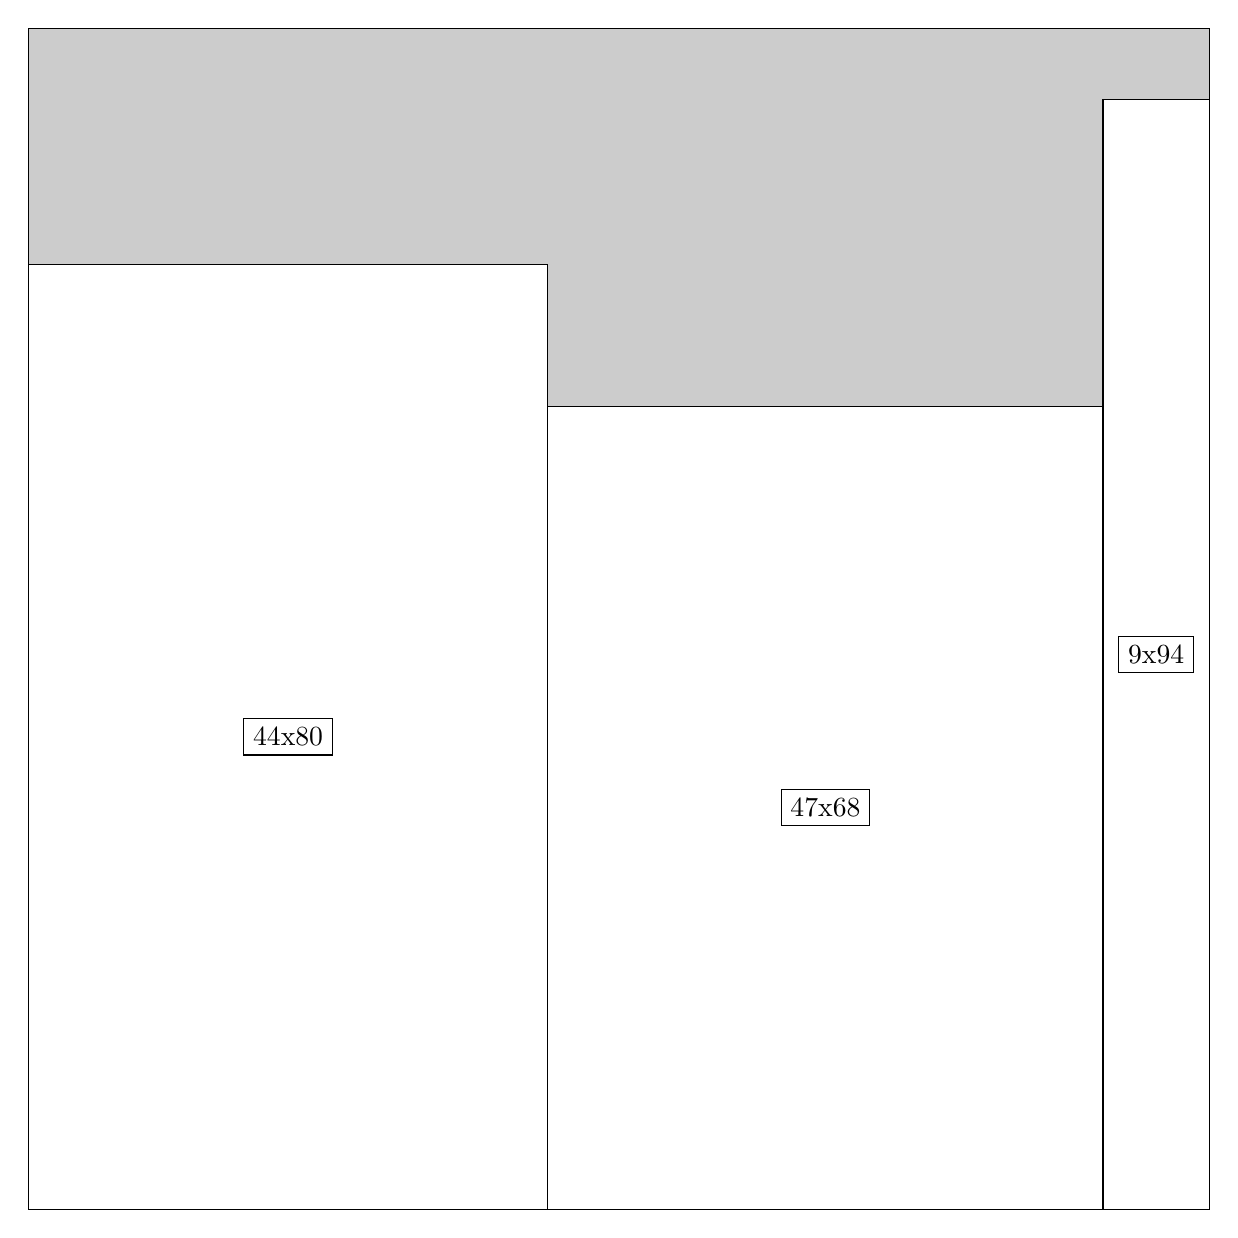
\begin{tikzpicture}[shorten >=1pt,scale=1.0,every node/.style={scale=1.0},->]
\tikzstyle{vertex}=[circle,fill=black!25,minimum size=14pt,inner sep=0pt]
\filldraw[fill=gray!40!white, draw=black] (0,0) rectangle (15.0,15.0);
\foreach \name/\x/\y/\w/\h in {44x80/0.0/0.0/6.6/12.0,47x68/6.6/0.0/7.05/10.2,9x94/13.65/0.0/1.3499999999999999/14.1}
\filldraw[fill=white!40!white, draw=black] (\x,\y) rectangle node[draw] (\name) {\name} ++(\w,\h);
\end{tikzpicture}


w =44 , h =80 , x =0 , y =0 , v =3520
\par
w =47 , h =68 , x =44 , y =0 , v =3196
\par
w =9 , h =94 , x =91 , y =0 , v =846
\par
\newpage


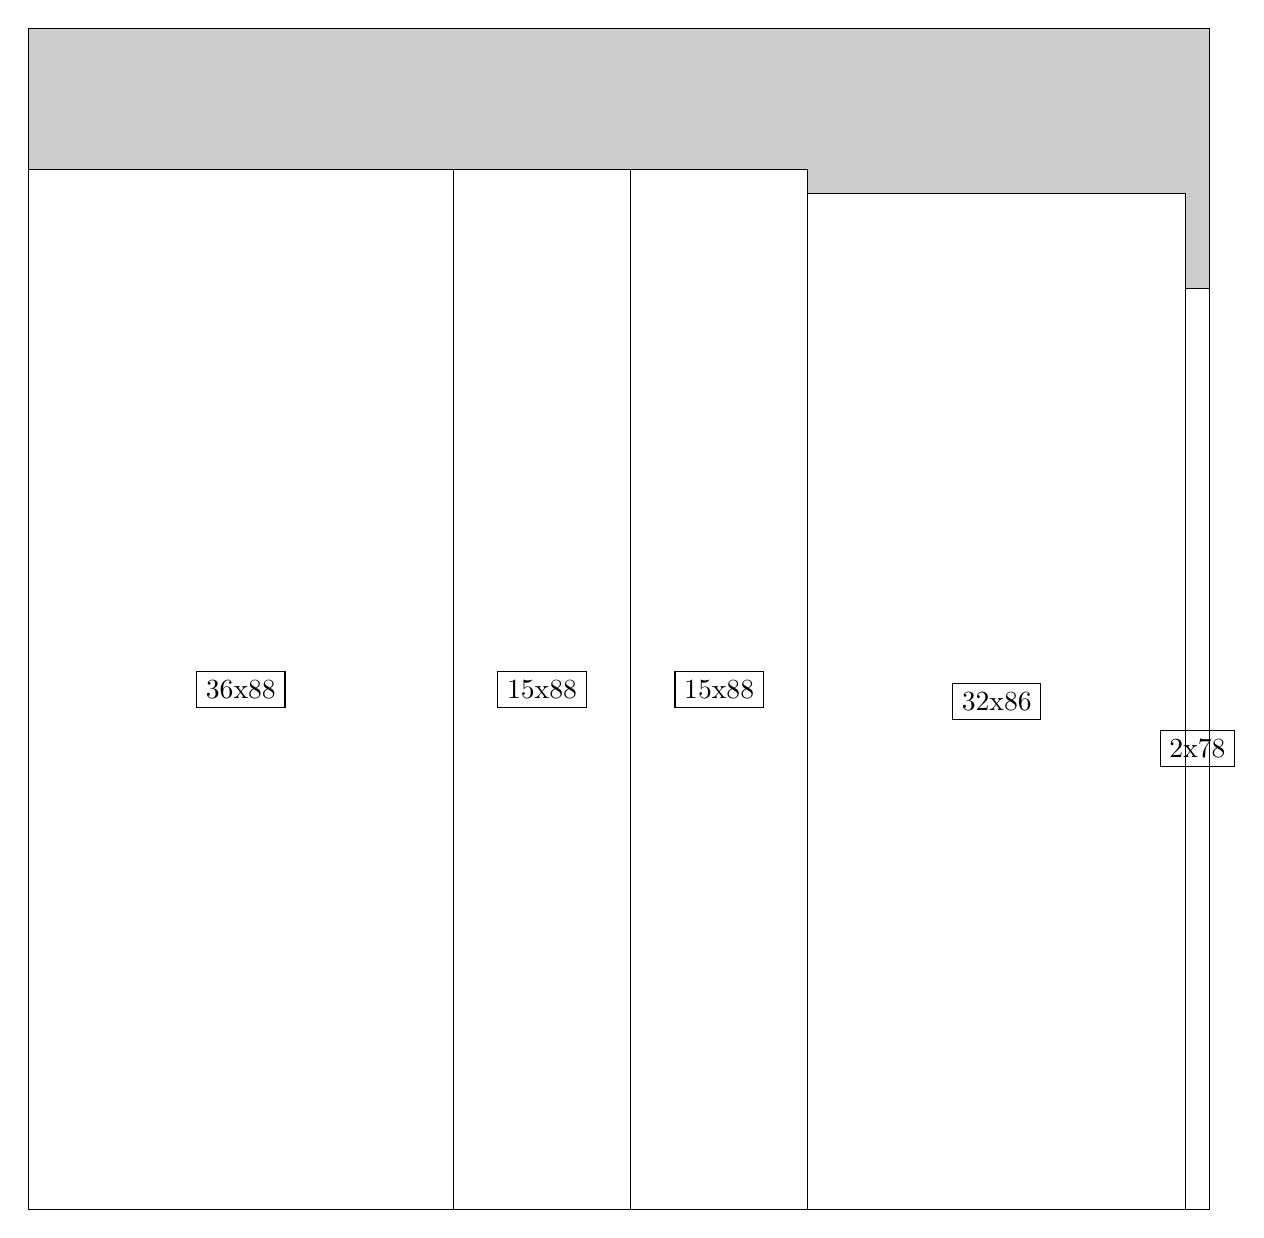
\begin{tikzpicture}[shorten >=1pt,scale=1.0,every node/.style={scale=1.0},->]
\tikzstyle{vertex}=[circle,fill=black!25,minimum size=14pt,inner sep=0pt]
\filldraw[fill=gray!40!white, draw=black] (0,0) rectangle (15.0,15.0);
\foreach \name/\x/\y/\w/\h in {36x88/0.0/0.0/5.3999999999999995/13.2,32x86/9.9/0.0/4.8/12.9,15x88/5.3999999999999995/0.0/2.25/13.2,15x88/7.6499999999999995/0.0/2.25/13.2,2x78/14.7/0.0/0.3/11.7}
\filldraw[fill=white!40!white, draw=black] (\x,\y) rectangle node[draw] (\name) {\name} ++(\w,\h);
\end{tikzpicture}


w =36 , h =88 , x =0 , y =0 , v =3168
\par
w =32 , h =86 , x =66 , y =0 , v =2752
\par
w =15 , h =88 , x =36 , y =0 , v =1320
\par
w =15 , h =88 , x =51 , y =0 , v =1320
\par
w =2 , h =78 , x =98 , y =0 , v =156
\par
\newpage


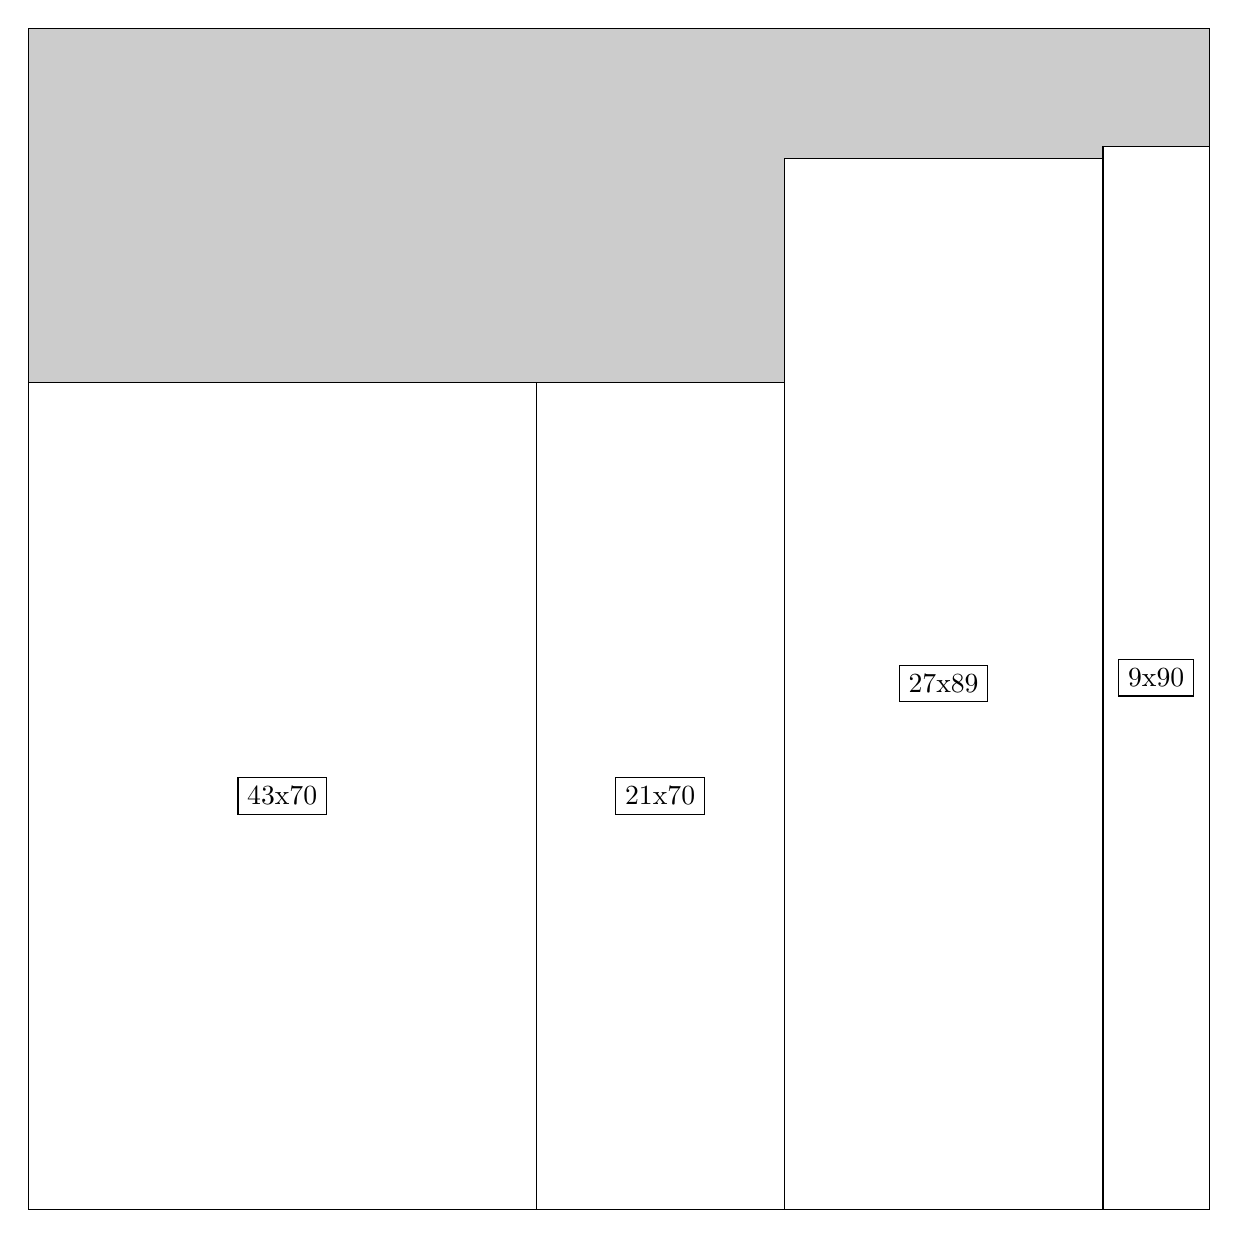
\begin{tikzpicture}[shorten >=1pt,scale=1.0,every node/.style={scale=1.0},->]
\tikzstyle{vertex}=[circle,fill=black!25,minimum size=14pt,inner sep=0pt]
\filldraw[fill=gray!40!white, draw=black] (0,0) rectangle (15.0,15.0);
\foreach \name/\x/\y/\w/\h in {43x70/0.0/0.0/6.45/10.5,27x89/9.6/0.0/4.05/13.35,21x70/6.45/0.0/3.15/10.5,9x90/13.65/0.0/1.3499999999999999/13.5}
\filldraw[fill=white!40!white, draw=black] (\x,\y) rectangle node[draw] (\name) {\name} ++(\w,\h);
\end{tikzpicture}


w =43 , h =70 , x =0 , y =0 , v =3010
\par
w =27 , h =89 , x =64 , y =0 , v =2403
\par
w =21 , h =70 , x =43 , y =0 , v =1470
\par
w =9 , h =90 , x =91 , y =0 , v =810
\par
\newpage


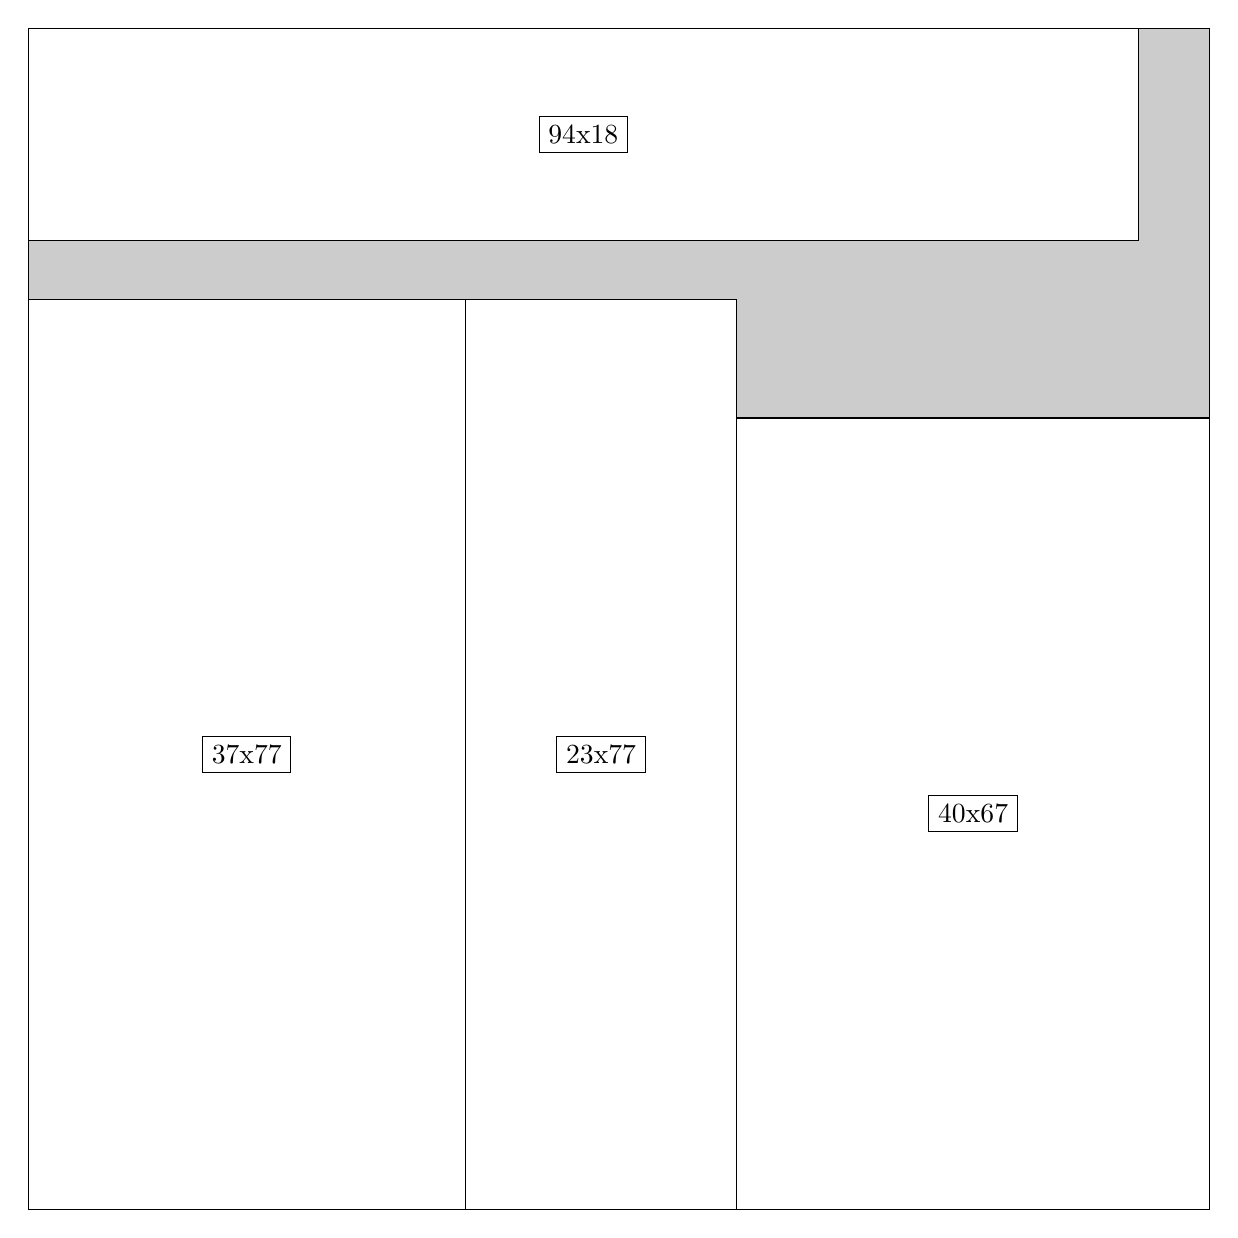
\begin{tikzpicture}[shorten >=1pt,scale=1.0,every node/.style={scale=1.0},->]
\tikzstyle{vertex}=[circle,fill=black!25,minimum size=14pt,inner sep=0pt]
\filldraw[fill=gray!40!white, draw=black] (0,0) rectangle (15.0,15.0);
\foreach \name/\x/\y/\w/\h in {37x77/0.0/0.0/5.55/11.549999999999999,40x67/9.0/0.0/6.0/10.049999999999999,23x77/5.55/0.0/3.4499999999999997/11.549999999999999,94x18/0.0/12.299999999999999/14.1/2.6999999999999997}
\filldraw[fill=white!40!white, draw=black] (\x,\y) rectangle node[draw] (\name) {\name} ++(\w,\h);
\end{tikzpicture}


w =37 , h =77 , x =0 , y =0 , v =2849
\par
w =40 , h =67 , x =60 , y =0 , v =2680
\par
w =23 , h =77 , x =37 , y =0 , v =1771
\par
w =94 , h =18 , x =0 , y =82 , v =1692
\par
\newpage


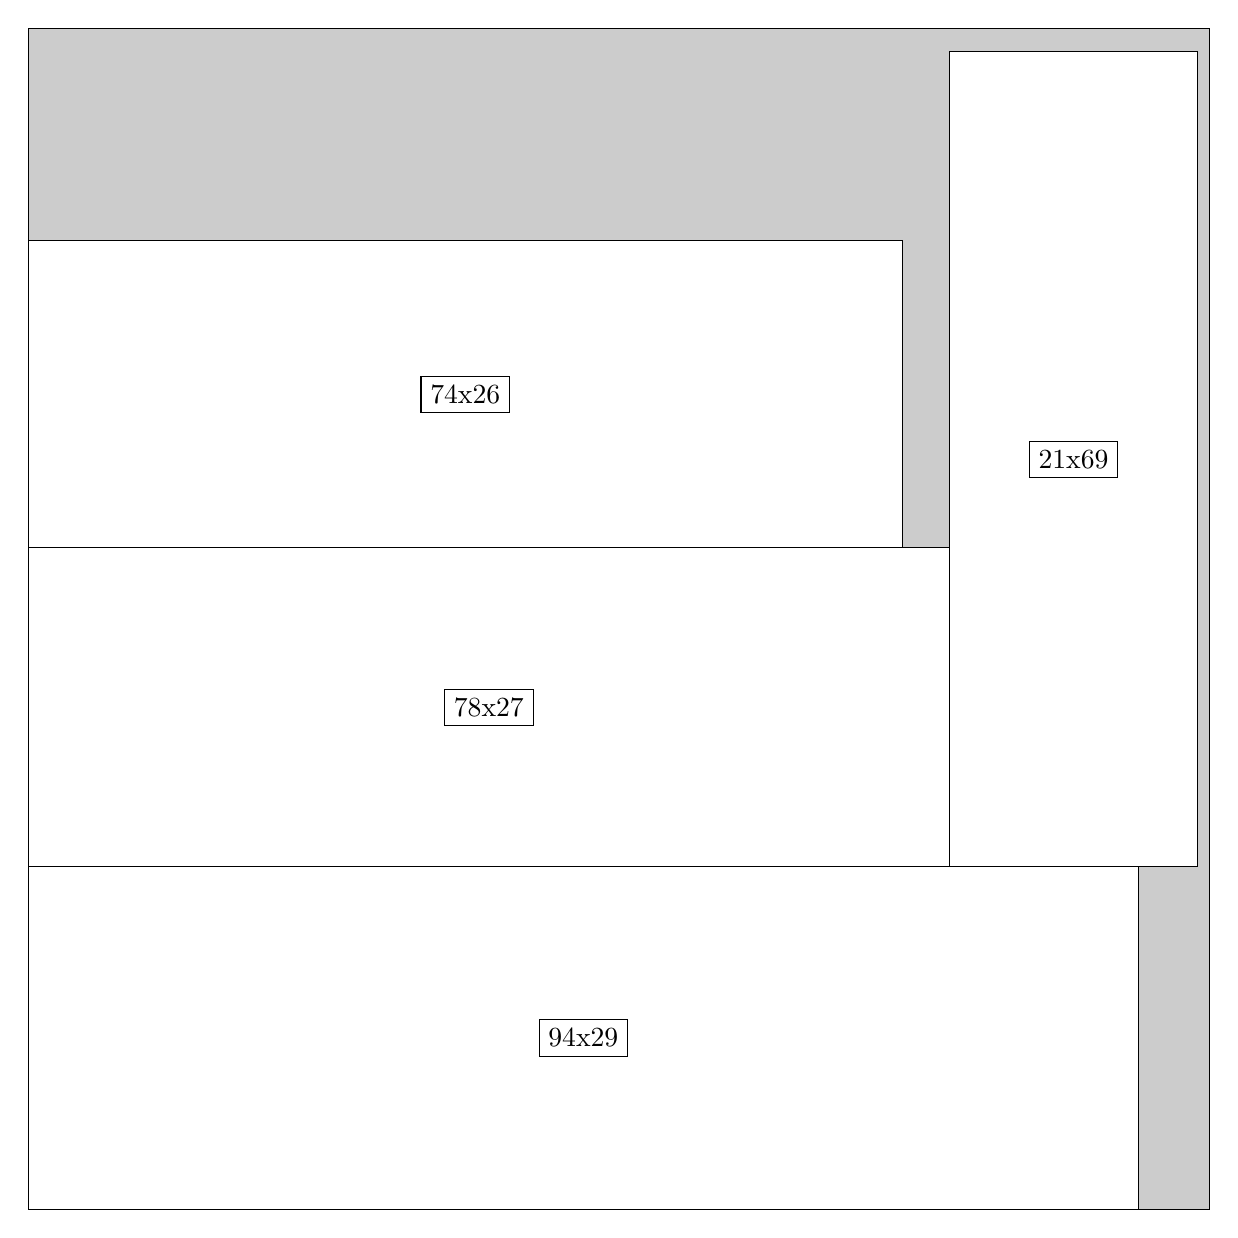
\begin{tikzpicture}[shorten >=1pt,scale=1.0,every node/.style={scale=1.0},->]
\tikzstyle{vertex}=[circle,fill=black!25,minimum size=14pt,inner sep=0pt]
\filldraw[fill=gray!40!white, draw=black] (0,0) rectangle (15.0,15.0);
\foreach \name/\x/\y/\w/\h in {94x29/0.0/0.0/14.1/4.35,78x27/0.0/4.35/11.7/4.05,74x26/0.0/8.4/11.1/3.9,21x69/11.7/4.35/3.15/10.35}
\filldraw[fill=white!40!white, draw=black] (\x,\y) rectangle node[draw] (\name) {\name} ++(\w,\h);
\end{tikzpicture}


w =94 , h =29 , x =0 , y =0 , v =2726
\par
w =78 , h =27 , x =0 , y =29 , v =2106
\par
w =74 , h =26 , x =0 , y =56 , v =1924
\par
w =21 , h =69 , x =78 , y =29 , v =1449
\par
\newpage


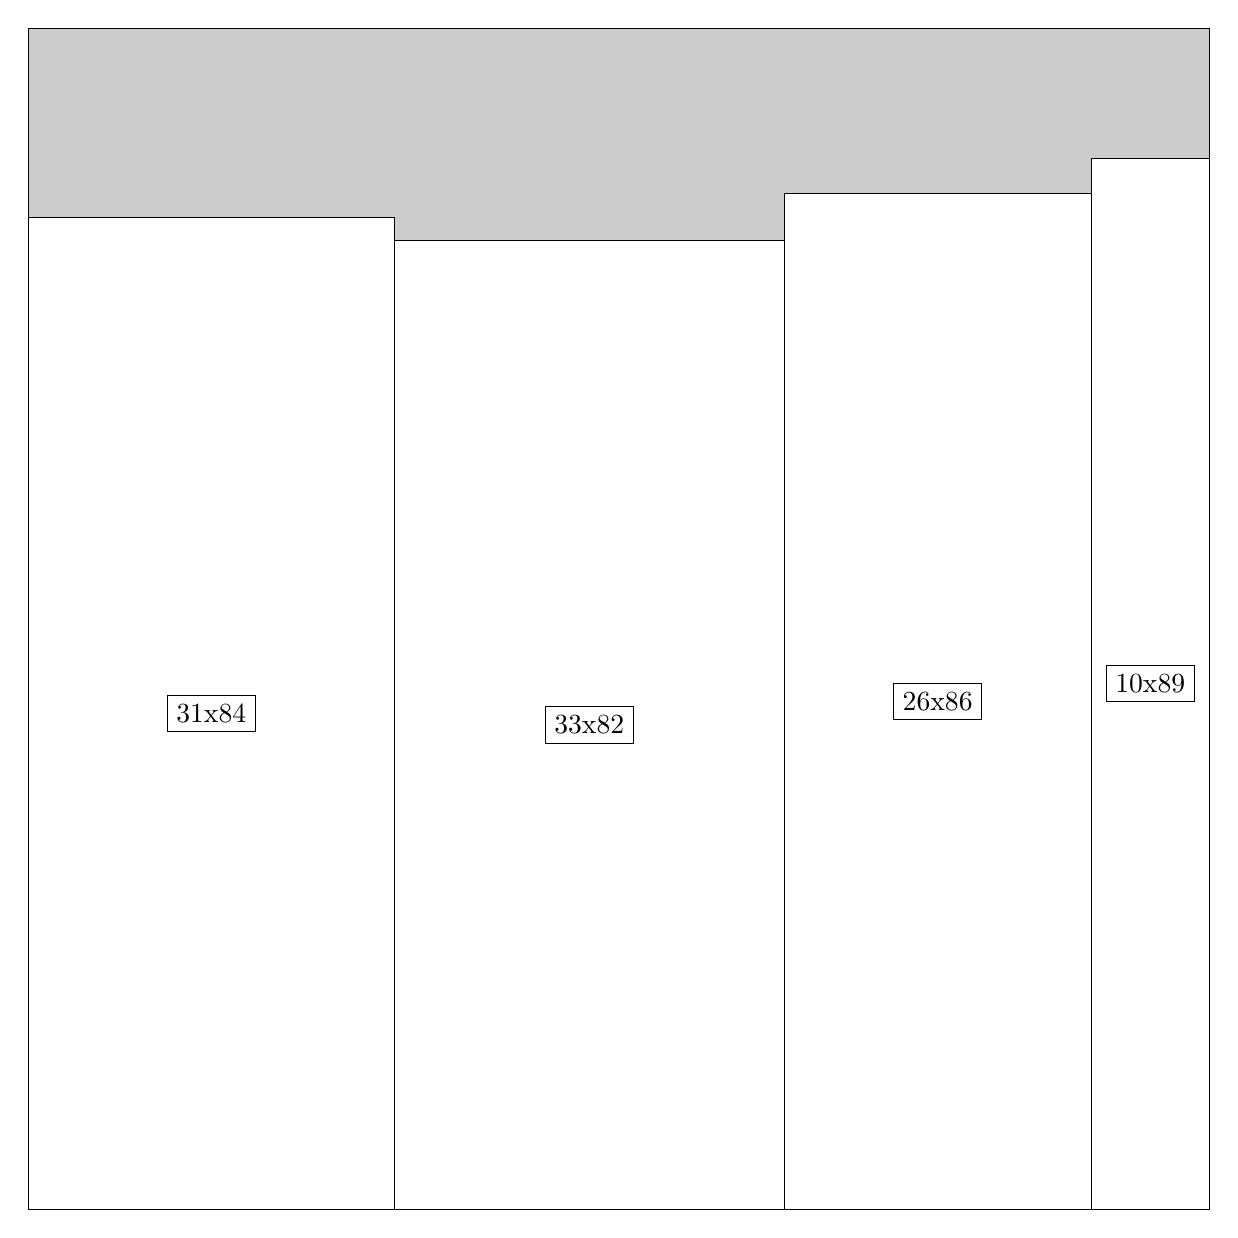
\begin{tikzpicture}[shorten >=1pt,scale=1.0,every node/.style={scale=1.0},->]
\tikzstyle{vertex}=[circle,fill=black!25,minimum size=14pt,inner sep=0pt]
\filldraw[fill=gray!40!white, draw=black] (0,0) rectangle (15.0,15.0);
\foreach \name/\x/\y/\w/\h in {31x84/0.0/0.0/4.6499999999999995/12.6,33x82/4.6499999999999995/0.0/4.95/12.299999999999999,26x86/9.6/0.0/3.9/12.9,10x89/13.5/0.0/1.5/13.35}
\filldraw[fill=white!40!white, draw=black] (\x,\y) rectangle node[draw] (\name) {\name} ++(\w,\h);
\end{tikzpicture}


w =31 , h =84 , x =0 , y =0 , v =2604
\par
w =33 , h =82 , x =31 , y =0 , v =2706
\par
w =26 , h =86 , x =64 , y =0 , v =2236
\par
w =10 , h =89 , x =90 , y =0 , v =890
\par
\newpage


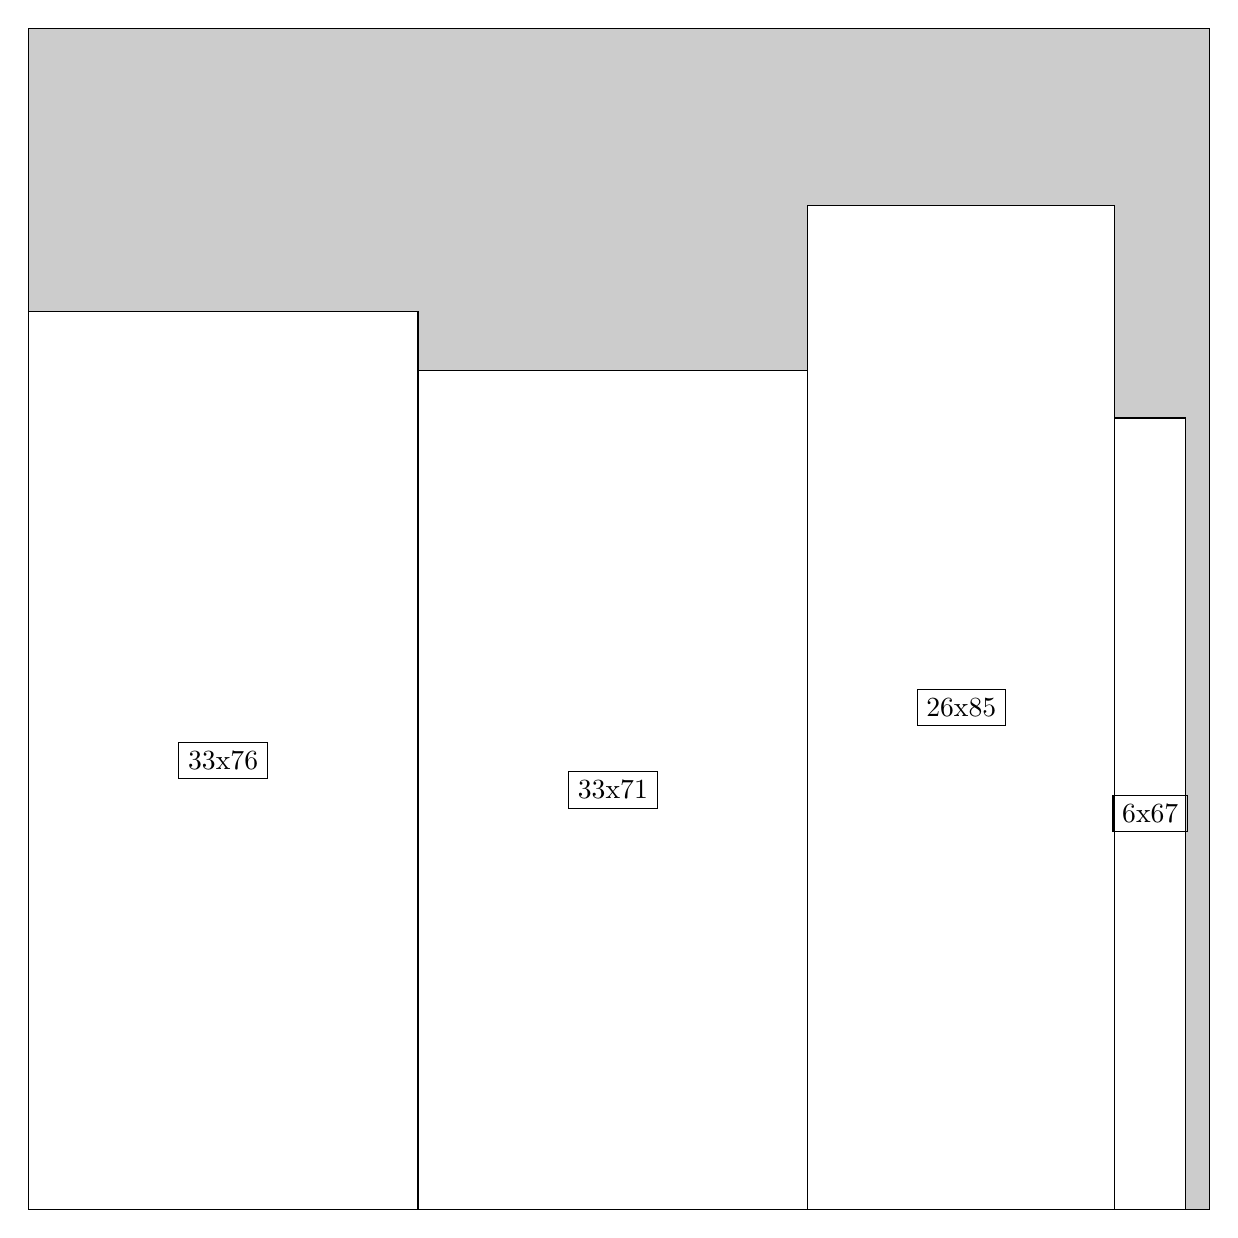
\begin{tikzpicture}[shorten >=1pt,scale=1.0,every node/.style={scale=1.0},->]
\tikzstyle{vertex}=[circle,fill=black!25,minimum size=14pt,inner sep=0pt]
\filldraw[fill=gray!40!white, draw=black] (0,0) rectangle (15.0,15.0);
\foreach \name/\x/\y/\w/\h in {33x76/0.0/0.0/4.95/11.4,33x71/4.95/0.0/4.95/10.65,26x85/9.9/0.0/3.9/12.75,6x67/13.799999999999999/0.0/0.8999999999999999/10.049999999999999}
\filldraw[fill=white!40!white, draw=black] (\x,\y) rectangle node[draw] (\name) {\name} ++(\w,\h);
\end{tikzpicture}


w =33 , h =76 , x =0 , y =0 , v =2508
\par
w =33 , h =71 , x =33 , y =0 , v =2343
\par
w =26 , h =85 , x =66 , y =0 , v =2210
\par
w =6 , h =67 , x =92 , y =0 , v =402
\par
\newpage


\end{document}